\documentclass[authoryear]{elsarticle}

\usepackage{amsmath}
\usepackage{bm}
\usepackage{tikz}
\usepackage{pgfplots}
\usepackage{color, colortbl}
\usepackage{graphicx}

\graphicspath{{figs/}}

\usepackage{hyperref}
\usepackage{multirow}

\newtheorem{thm}{Theorem}
\newtheorem{lem}[thm]{Lemma}
\newproof{pf}{Proof}

\journal{Annals of Nuclear Energy}

\bibliographystyle{elsarticle-harv}

\begin{document}

\begin{frontmatter}

\title{Numerical modeling of neutron transport in $\mathrm{SP_3}$ approximation by finite element method}

\author[ki]{Alexander V. Avvakumov}
\ead{Avvakumov2009@rambler.ru}

\author[nsi]{Valery~F.~Strizhov}
\ead{vfs@ibrae.ac.ru}

\author[nsi,univ]{Petr N. Vabishchevich\corref{cor}}
\ead{vabishchevich@gmail.com}

\author[univ]{Alexander O. Vasilev}
\ead{haska87@gmail.com}

\address[ki]{National Research Center \emph{Kurchatov Institute},  1, Sq. Academician Kurchatov, Moscow, Russia}
\address[nsi]{Nuclear Safety Institute, Russian Academy of Sciences, 52, B. Tulskaya, Moscow, Russia}
\address[univ]{North-Eastern Federal University, 58, Belinskogo, Yakutsk, Russia}

\cortext[cor]{Corresponding author}

\begin{abstract}
The $\mathrm{SP_3}$ approximation of the neutron transport equation allows improving the accuracy for both static and transient simulations for reactor core analysis compared with the neutron diffusion theory. 
Besides, the $\mathrm{SP_3}$ calculation costs are much less than higher order transport methods ($\mathrm{S_N}$ or $\mathrm{P_N}$). 
Another advantage of the $\mathrm{SP_3}$ approximation is a similar structure of equations that is used in the diffusion method. 
Therefore, there is no difficulty to implement the $\mathrm{SP_3}$ solution option to the multi-group neutron diffusion codes. 
In this work, the application of the $\mathrm{SP_3}$ methodology based on solution of the $\lambda$- and $\alpha$-spectral problems has been tested for the IAEA-2D and HWR reactor benchmark tests. 
The FEM is chosen to achieve the 3D geometrical generality, using GMSH as a generic mesh generator. 
The results calculated with the diffusion and $\mathrm{SP_3}$ methods are compared with the reference transport calculation results. 
It was found for the HWR reactor test that some eigenvalues are complex when calculating using both diffusion and $\mathrm{SP_3}$ options.
\end{abstract}

\begin{keyword}
neutron transport equation, diffusion theory, $\mathrm{SP_3}$ approximation, reactor core, spectral problems, eigenvalues.

\end{keyword}

\end{frontmatter}

\section{Introduction}
The diffusion approximation of the neutron transport equation is widely used in nuclear reactor analysis allowing whole-core calculations with reasonable accuracy. 
The main feature of neutron diffusion equation is following: it is assumed that the neutron current is proportional to the neutron flux gradient (the Fick’s law). 
There are also three assumptions: neutron absorption much less likely than scattering, linear spatial variation of the neutron distribution and isotropic scattering \citep{stacey2007}. 
To provide the validity of diffusion theory, the modern diffusion codes use, as a rule, assembly-by-assembly coarse-mesh calculation scheme with effective homogenized cross sections, prepared by more accurate transport approximations. 
To improve the diffusion code restrictions related with limitations on mesh spacing, different approaches are used including nodal and finite element methods \citep{avvakumov2017spectral, lawrence1986progress}.

For many situations of interest (for instance, the pin-by-pin calculation taking account strongly absorbing control rods), the applicability of neutron diffusion theory are limited. 
Therefore, a more rigorous approximation for the neutron transport is required.

The solution of the neutron transport equation is very complicated problem because of seven independent variables: five for space-angular description, one for energy and one for time. 
To simplify the transport problem, different approaches are used such as the spherical harmonics ($\mathrm{P_N}$) approximation \citep{azmy2010nuclear}. 
The $\mathrm{P_N}$ approximation of the neutron transport equation is derived by expansion of the angular dependence of the neutron flux in the N spherical harmonics. 
During the last time, the simplest version of the $\mathrm{P_N}$ method, namely the simplified $\mathrm{P_N}$ approximation became widespread \citep{mcclarren2010theoretical}. 
The major feature of the $\mathrm{SP_N}$ method is following: the three-dimensional neutron transport equation is transformed to a set of one-dimensional equations. 
The number of the $\mathrm{SP_N}$ trial functions is equal to 2(N+1) compared with the $\mathrm{P_N}$ method which uses (N+1)$^2$ trial functions. 
This leads to significant reduce in the computation time for typical whole-core calculations. 

The $\mathrm{SP_N}$ approximation was first derived by Gelbard \citep{gelbard1960application, gelbard1961simplified, gelbard1962applications} in the early 1960s. 
He replaced the spatial derivatives with Laplacian and divergence operators in a one-dimensional planar geometry. 
The resulting $\mathrm{SP_N}$ equations are elliptic, for example, the $\mathrm{SP_3}$ equations consist of two equations of diffusion type with two unknown fluxes: the scalar flux and the second angular flux moment. 
More rigorous theoretical foundation of the $\mathrm{SP_3}$ methodology has been derived by Brantley and Larsen \citep{brantley2000simplified} on the basis of variational methods.

The $\mathrm{SP_3}$ method, as expected, can provide accuracy improvement compared with the common used diffusion method. 
Besides, implementation of the $\mathrm{SP_3}$ equations into the diffusion code is not difficult because of the similar structure of the $\mathrm{SP_3}$ and diffusion equations. 
For this reason the $\mathrm{SP_3}$ method was adopted in different whole-core calculation codes, such as DYN3D \citep{beckert2008development}, PARCS \citep{downar2010theory} and others. According to \citep{tada2008applicability}, application of the $\mathrm{SP_3}$ theory to the pin-by-pin calculation for BWR geometry resulted in remarkable improvement in the calculation accuracy compared with the diffusion method. 
Besides, as it turned out, the computation time using the $\mathrm{SP_3}$ method is only 1.5 times longer than that using the diffusion method \citep{tada2008applicability}.

Thus, the $\mathrm{SP_3}$ method can be considered as an improved approximation of the neutron transport equation compared with the diffusion method. 
In this regard, it will be very useful to compare the spectral parameters, calculated by both the diffusion and $\mathrm{SP_3}$ methods. 
To characterize the reactor steady-state conditions or dynamic behavior, some spectral problems are considered \citep{stacey2007, bell1970}. 
The steady-state condition is usually described by solution of a spectral problem ($\lambda$-eigenvalue problem); the fundamental eigenvalue (the largest eigenvalue) is called k-effective of the reactor core \citep{stacey2007, bell1970}. 
The reactor dynamic behavior can naturally be described on the basis of the approximate solution expansion in time-eigenvalue of $\alpha$-eigenvalue problem \citep{ginestar2002transient, verdu20103d, verdu2014modal}. 
At large times, one can talk about the asymptotic behavior of a neutron flux, whose amplitude is exp($\alpha$t). 
Previously the complex eigenvalues and eigenfunctions were found in the spectral problems for some numerical tests \citep{avvakumov2017spectral}.

In this paper we consider the $\mathrm{SP_N}$ approximation for the steady-state multi-group neutron transport problem.
To solve spectral problems with nonsymmetrical matrices we use well-designed algorithms and relevant free software including the library SLEPc (Scalable Library for Eigenvalue Problem Computations, http://slepc.upv.es/). 
We use a Krylov-Schur algorithm, a variation of Arnoldi method, described in \citep{stewart2002krylov}.

The paper is organized as follows. 
The steady-state and dynamic models of a nuclear reactor based on the multigroup $\mathrm{SP_3}$ equations are given in Section 2. 
In Section 3 we discuss various spectral problems. 
Some numerical examples of calculation of spectral characteristics of two-dimensional test problems for IAEA-2D benchmark problem and HWR reactor using the two-group system of diffusion and $\mathrm{SP_3}$ equations is discussed in Section 4. 
The results of the work are summarized in Section 5.

\section{Problem statement}
Let’s consider the symmetric form of the $\mathrm{SP_3}$ equation for the neutron flux \citep{ryu2010development}.
The neutron dynamics is considered in the limited convex two-dimensional or three-dimensional area  $\Omega$ ($\bm x = \{x_1, ..., x_d\} \in \Omega, \ d = 2,3$) with boundary $\partial \Omega$. 
The neutron transport is described by the system of equations
\begin{equation}\label{1.1}
\begin{split}
 \frac{1}{v_g} \frac{\partial \phi_{0,g}}{\partial t} - \frac{2}{v_g} \frac{\partial \phi_{2,g}}{\partial t} - & \nabla \cdot D_{0,g} \nabla \phi_{0,g} + \Sigma_{r,g} \phi_{0,g} -  2\Sigma_{r,g} \phi_{2,g} = \\ 
 =  & (1-\beta)\chi_{n,g} S_{n} + S_{s,g} + \chi_{d,g} S_d, \\
 -\frac{2}{v_g} \frac{\partial \phi_{0,g}}{\partial t} + \frac{9}{v_g} \frac{\partial \phi_{2,g}}{\partial t} - & \nabla \cdot D_{2,g} \nabla \phi_{2,g} + (5\Sigma_{t,g} + 4\Sigma_{r,g}) \phi_{2,g} - 2\Sigma_{r,g} \phi_{0,g} = \\ 
 =  & -2(1-\beta)\chi_{n,g} S_{n} - 2S_{s,g} - 2\chi_{d,g} S_d,
\end{split}
\end{equation}
where
\[
S_{n} =  \sum_{g'=1}^{G} \nu \Sigma_{f,g'} \phi_{g'}, 
\quad
S_{s,g} = \sum_{g\neq g'=1}^{G} \Sigma_{s,g'\rightarrow g} \phi_{g'},
\quad
S_{d} = \sum_{m=1}^{M} \lambda_m c_m,
\]
\[
\phi_{0,g}=\phi_g + 2\phi_{2,g}, 
\quad
D_{0,g} = \cfrac{1}{3\Sigma_{tr,g}}, 
\quad
D_{2,g} = \cfrac{9}{7\Sigma_{t,g}}, 
\quad g=1,2,...,G.
\]
Here $G$ --- number of energy groups,
$\phi_g(\bm x, t)$ --- scalar flux,
$\phi_{0,g}(\bm x, t)$ --- pseudo 0th moment of angular flux,
$\phi_{2,g}(\bm x, t)$ --- second moment of angular flux,
$\Sigma_{t,g}(\bm x, t)$ --- total cross-section, 
$\Sigma_{tr,g}(\bm x, t)$ --- transport cross-section, 
$\Sigma_{r,g}(\bm x, t)$ --- removal cross-section,
$\Sigma_{s,g'\rightarrow g}(\bm x, t)$ --- scattering cross-section,
$\chi_g$  --- spectra of neutrons, 
$\nu\Sigma_{f,g}(\bm x, t)$ --- generation cross-section,
$c_m(\bm x, t)$ --- density of sources of delayed neutrons,
$\lambda_m$ --- decay constant of sources of delayed neutrons,
$M$ --- number of types of delayed neutrons.

The density of sources of delayed neutrons is described by the equations
\begin{equation}\label{1.2}
 \frac{\partial c_m}{\partial t} + \lambda_m c_m = \beta_m S_{n},
 \quad m = 1,2, ..., M, 
\end{equation}
where $\beta_m$ is a fraction of delayed neutrons of m-type, and
\[
 \beta = \sum_{m=1}^{M} \beta_m.
\] 
The Marshak-type conditions are set at the boundary of the area $\partial \Omega$
\begin{equation}\label{1.3}
\begin{split}
\begin{bmatrix}
J_{0,g}(\bm x)\\
J_{2,g}(\bm x)\\
\end{bmatrix}
=
\begin{bmatrix}
\phantom{-}\cfrac{1}{2} & -\cfrac{3}{8} \\
 -\cfrac{3}{8} & \phantom{-}\cfrac{21}{8} \\
\end{bmatrix}
\begin{bmatrix}
\phi_{0,g}(\bm x) \\
\phi_{2,g}(\bm x) \\
\end{bmatrix},
\quad
J_{i,g}(\bm x) = -D_{i,g}\nabla\phi_{i,g}(\bm x), 
\quad
i = 0, 2.
\end{split}
\end{equation}

System of equations (\ref{1.1}) and (\ref{1.2}) is supplemented with boundary conditions (\ref{1.3}) and corresponding initial conditions
\begin{equation}\label{1.4}
 \phi_g(\bm x,0) = \phi_g^0(\bm x), 
 \quad g = 1,2, ..., G,
 \quad c_m(\bm x,0) = c_m^0(\bm x), 
 \quad m = 1,2, ..., M.
\end{equation}

Let's write the boundary problem (\ref{1.1})--(\ref{1.4}) in operator form. 
The vectors $\bm u_1 = \{\phi_{0,1}, \phi_{0,2}, \cdots, \phi_{0,G}\}$, $\bm u_2 = \{\phi_{2,1}, \phi_{2,2}, \cdots, \phi_{2,G}\}$, $\bm c = \{c_1, c_2, ..., c_M\}$ and matrices are defined as follows
\[
V = (\mathrm{v}_{gg'}),
\enskip
\mathrm{v}_{gg'} = \frac{1}{v_g} \delta_{gg'},
\quad
B = (b_{gg'}),
\enskip
b_{gg} = -2\Sigma_{r,g},
\enskip
b_{gg'} = 2\Sigma_{s, g' \rightarrow g},
\]
\[
A_1 = (a_{gg'}),
\enskip
a_{gg} = -\nabla \cdot D_{0,g} \nabla + \Sigma_{r,g},
\enskip
a_{gg'} = -\Sigma_{s, g' \rightarrow g},
\]
\[
A_2 = (a_{gg'}),
\enskip
a_{gg} = -\nabla \cdot D_{2,g} \nabla + 5\Sigma_{tr,g} + 4\Sigma_{r,g},
\enskip
a_{gg'} = -4\Sigma_{s, g' \rightarrow g},
\]
\[
F = (f_{gg'}),
\enskip
f_{gg'} = \chi_{n,g}\nu\Sigma_{f,g'},
\quad
E =(e_{gm}),
\enskip
e_{gm} = \chi_{d,g}\lambda_m,
\]
\[
\Lambda = (\lambda_{mm'}), 
\enskip
\lambda_{mm'} = \delta_{mm'}\lambda_m,
\quad
Q = (q_{mg}),
\enskip
q_{mg} =\beta_m \nu\Sigma_{f,g},
\]
where
\[
 \delta_{g g'} = \left \{ 
 \begin{matrix}
 1, & g = g', \\
 0, & g \neq  g',
 \end{matrix}
 \right. 
\]  
is the Kronecker symbol.
We shall use the set of vectors $\bm u$, whose components satisfy the boundary conditions (\ref{1.3}). 
Using the set definitions, the system of equations (\ref{1.1}) and (\ref{1.2}) can be written as following
\begin{equation}\label{1.5}
\begin{split}
V (\frac{\partial \bm u_1}{\partial t} - 2 \frac{\partial \bm u_2}{\partial t}) + A_1 \bm u_1 + B \bm u_2 &=(1-\beta) F (\bm u_1 - 2\bm u_2) + E\bm c,
\\
V(- 2 \frac{\partial \bm u_1}{\partial t} + 9 \frac{\partial \bm u_2}{\partial t} ) + A_2 \bm u_2 + B \bm u_1 &=-2(1-\beta) F (\bm u_1 - 2\bm u_2) - 2E\bm c,
\\
\frac{\partial \bm c}{d t} + \Lambda \bm c &= Q (\bm u_1 - 2\bm u_2). 
\end{split}
\end{equation}
Without taking into account delayed neutrons, we have
\begin{equation}\label{1.6}
\begin{split}
V (\frac{\partial \bm u_1}{\partial t} - 2 \frac{\partial \bm u_2}{\partial t}) + A_1 \bm u_1 + B \bm u_2 &= F (\bm u_1 - 2\bm u_2),
\\
V( - 2 \frac{\partial \bm u_1}{\partial t} + 9 \frac{\partial \bm u_2}{\partial t}) + A_2 \bm u_2 + B \bm u_1 &=-2 F (\bm u_1 - 2\bm u_2).
\end{split}
\end{equation}
The Cauchy problem is formulated for equations (\ref{1.5}) and (\ref{1.6}) when
\begin{equation}\label{1.7}
 \bm u_1(0) = \bm u_1^0, \quad  \bm u_2(0) = \bm u_2^0, \quad \bm c(0) = \bm c^0,
\end{equation} 
where $\bm u_1^0 = \{\phi_{0,1}^0,  \phi_{0,2}^0, ...,  \phi_{0,G}^0 \}$, 
$\bm u_2^0 = \{\phi_{2,1}^0,  \phi_{2,2}^0, ...,  \phi_{2,G}^0 \}$ and 
$\bm c^0 = \{ c_1^0,  c_2^0, ...,  c_M^0 \}$.

\section{Spectral problems}
To characterize the reactor dynamic processes described by
Cauchy problem (\ref{1.5})-(\ref{1.7}), let’s consider some spectral problems \citep{bell1970,stacey2007}.

The spectral problem, which is known as the $\lambda$-spectral problem, is usually considered.
For the system of equations (\ref{1.6}), (\ref{1.7}), we have
\begin{equation}\label{1.8}
L \bm \varphi = \lambda^{(k)} M \bm \varphi,
\end{equation}
where
\[
\bm \varphi = \{\bm \varphi_1, \bm \varphi_2\},
\quad
L = \begin{pmatrix}
A_1 & B \\
B & A_2 \\
\end{pmatrix},
\quad
M = \begin{pmatrix}
F & -2F \\
-2F & 4F \\
\end{pmatrix}.
\]
The minimal eigenvalue is used for characterisation of neutron field, thus
\[
 k = \frac{1}{\lambda^{(k)}_1}  
\] 
is the effective multiplication factor (k-effective).
The value $k = \lambda^{(k)}_1 = 1$ is related to the critical state of the reactor, and the corresponding eigenfunction $\bm{\varphi}^{(1)}(\bm x)$ is the stationary solution of the Eq (\ref{1.5}), (\ref{1.6}).
At $k > 1$, one can speak about supercriticality, at $k < 1$ --- about subcriticality.

%Due to nonself-adjoint operators of neutron transport we have, generally speaking, the complex eigenvalues. The reality and positivity property of the fundamental eigenvalue for the system of neutronics equations is proved using the principle of maximum at some restrictions on factors of neutron transport operators (Habetler and Martino, 1961). This is also true for the nonself-adjoint elliptic operator of the second order (Evans, 1998).

The spectral problem (\ref{1.8}) cannot directly be connected with the
dynamic processes in a nuclear reactor. 
The eigenvalues of the multiplication factor of the reactor and the corresponding eigenfunctions do not depend on the time delay for the emission of delayed neutrons. 
The reason is that the problem (\ref{1.8}) on eigenvalues ​​is the problem of finding time-independent solutions of the neutron transport equation, and the term describing the contribution of fission to the neutron balance is equal to the total number of fission neutrons, both instantaneous and delayed divided by $k$.
At the best, we can get only the limiting case --- the stationary critical state.
The more acceptable spectral characteristics for the non-stationary equation (\ref{1.5}) are related the spectral problem
\begin{equation}\label{1.9}
\begin{split}
L \bm \varphi - (1 - \beta) M \bm \varphi - I \bm s &= \lambda^{(\alpha)} W \bm \varphi, \\
\Lambda \bm s - R \bm \varphi  &= \lambda^{(\alpha)} \bm s.
\end{split}
\end{equation}
Without taking into account delayed neutrons (\ref{1.6}), we have
\begin{equation}\label{1.10}
L \bm \varphi - M \bm \varphi = \lambda^{(\alpha)} W \bm \varphi,
\end{equation}
where
\[
I = \begin{pmatrix}
E \\
-2E \\
\end{pmatrix},
\quad
R = \begin{pmatrix}
Q & -2Q \\
\end{pmatrix},
\quad
W = \begin{pmatrix}
V & -2V \\
-2V & 9V \\
\end{pmatrix}
\]
The fundamental eigenvalue
\[ 
 \alpha = \lambda^{(\alpha)}_1
\]
is called \citep{bell1970} $\alpha$-eigenvalues or period eigenvalues, because they are inversely related to the reactor periods.
The problem of the period eigenvalues essentially takes into account the contribution of delayed neutrons.
In particular, the long lifetime of the predecessors of delayed neutrons makes a large contribution to the slowly decreasing eigenfunctions of the reactor period, and this does not occur when only instantaneous neutrons are taken into account.

The asymptotic behaviour of Cauchy problem solution (\ref{1.5})-(\ref{1.7}) at large times can be connected with the eigenvalue $\alpha$.
In this regular mode, the reactor behaviour is described by the function $\exp(-\alpha t) \bm \varphi^{(1)}(\bm x)$.
Critical state of the reactor is defined by the values $\alpha = 0$; when $\alpha > 0$ we get the supercritical state, and when $\alpha <  0$ --- subcritical state of the reactor.

\section{Numerical examples}
We shall give some results of eigenvalue calculation. 
The elementary two-group model ($G = 2$) is used. 
The method of finite elements \citep{brenner2008, quarteroni2008} on triangular calculation grids is used for the approximate solution of the spectral problem. 
The standard Lagrangian finite elements are used.
The software has been developed using the engineering and scientific calculation library FEniCS \citep{logg2012}.
SLEPc has been used for numerical solution of the spectral problems.
We used a Krylov-Schur algorithm with an accuracy of $10^{-15}$.
The following parameters were varied in the calculations:
\begin{itemize}\itemsep1pt \parskip0pt \parsep0pt
\item $n$ --- the number of triangles per one assembly (Fig.~\ref{fig:mesh}); 
\item $p$ --- the order of finite element.
\end{itemize}
We compare the calculations based on the $\mathrm{SP_3}$ model and the diffusion model  in \citep{avvakumov2014, avvakumov2017spectral}.


\begin{figure}[htp]
	\begin{minipage}{0.30\linewidth}
		\center{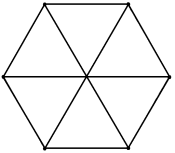
\includegraphics[width=1\linewidth]{mesh1.png}}\\
	\end{minipage}
	\hfill
	\begin{minipage}{0.30\linewidth}
		\center{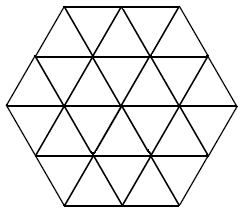
\includegraphics[width=1\linewidth]{mesh2.png}}\\
	\end{minipage}
	\hfill
	\begin{minipage}{0.30\linewidth}
		\center{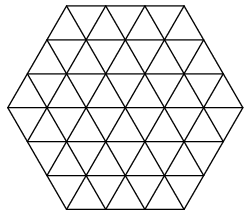
\includegraphics[width=1\linewidth]{mesh3.png}}\\
	\end{minipage}
	\caption{Discretization of assembly into 6, 24 and 96 finite elements.}
	\label{fig:mesh}
\end{figure}

\subsection{IAEA-2D without reflector}
The test problem for reactor IAEA-2D without reflector \citep{chao1995} in two-dimensional approximation ($\Omega$ is the section of reactor core) is considered.
The geometrical model of the IAEA-2D reactor core consists of a set of hexagonal assemblies and is presented in Fig.~\ref{fig:iaea}, where the assemblies of various types are marked with various digits. 
The total size of assembly equals 20 cm. 

\begin{figure}[htp]
	\center{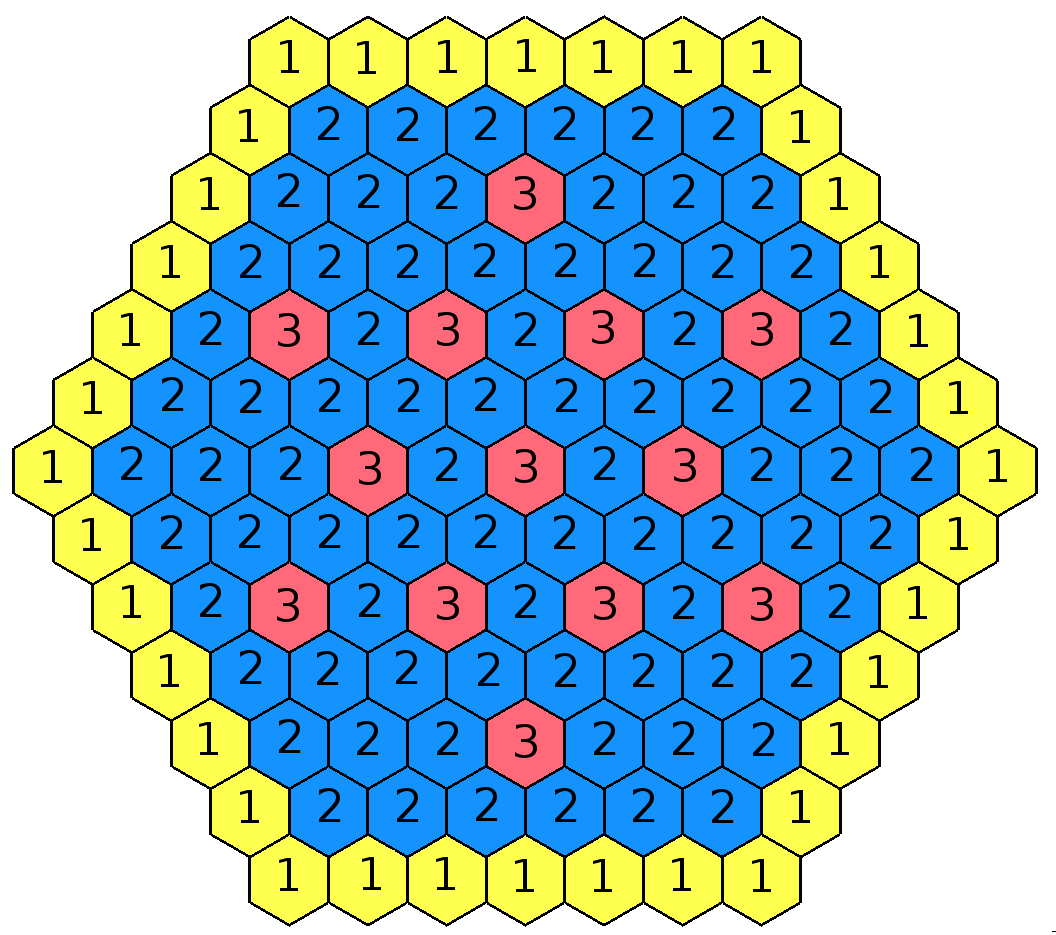
\includegraphics[width=0.6\linewidth]{iaea.png}}\\
	\caption{Geometrcial model of the IAEA-2D reactor core without reflector.}
	\label{fig:iaea}
\end{figure}

Diffusion neutronics constants in the common units are given in Table~\ref{tab:iaea}.
The following delayed neutrons parameters are used: one group of delayed neutrons with effective fraction $\beta_1 = 6.5\cdot10^{-3}$ and decay constant $\lambda_1 = 0.08$ s$^{-1}$. 
Neutron velocity  $v_1 = 1.25 \cdot 10^7$ cm/s and $v_2 = 2.5 \cdot 10^5$ cm/s.

\begin{table}[htp]
\caption{Diffusion neutronics constants for IAEA-2D.}
\label{tab:iaea}
\begin{center}
\begin{tabular}{c l l l l l}
\hline
Material & 1 & 2 & 3 & 4\\
\hline 
$D_1$ & 1.5 & 1.5 & 1.5 & 1.5\\
$D_2$ & 0.4 & 0.4 & 0.4 & 0.4\\
$\Sigma_{a1}$ & 0.01 & 0.01 & 0.01 & 0.0\\
$\Sigma_{a2}$ & 0.08 & 0.085 & 0.13 & 0.01\\
$\Sigma_{s,1\rightarrow2}$ & 0.02 & 0.02 & 0.02 & 0.04\\
$\Sigma_{s,1\rightarrow1}$ & 0.1922222 & 0.1922222 & 0.1922222 & 0.1822222\\
$\Sigma_{s,2\rightarrow2}$ & 0.7533333 & 0.7483333 & 0.7033333 & 0.8233333\\
$\nu_1\Sigma_{f1}$ & 0.00 & 0.00 & 0.00 & 0.00\\
$\nu_2\Sigma_{f2}$ & 0.135 & 0.135 & 0.135 & 0.00\\
\hline
\end{tabular}
\end{center}
\end{table}

\subsubsection{Solution of Lambda Modes spectral problem}
The obtained results by \citep{avvakumov2014} was taken as a reference solution for the diffusion model, and for the $\mathrm{SP_3}$ model --- the solution on a fine grid with $p = 3, n = 96$.
The results of the solution of the effective multiplication factor for test IAEA-2D without a reflector are shown in Table~\ref{tab:iaea_without_lambda}.
Hereinafter, for $\lambda$-spectral problems, the following notation is used: $k_{dif}$ --- effective multiplication factor by diffusion model; $k_{sp_3}$ --- effective multiplication factor by $\mathrm{SP_3}$ model; $\Delta$ --- absolute deviation from the reference value in pcm ($10^{-5}$); $\delta$ --- the standard deviation of the relative power. %%$t$ --- время счета.

\begin{table}[htp]
\caption{The effective multiplication factor.}
\label{tab:iaea_without_lambda}
\begin{center}
\begin{tabular}{c r r r r r r r}
\hline
$n$ & $p$ & $k_{dif}$ & $\Delta_{dif}$ & $\delta_{dif}$ &$k_{sp_3}$& $\Delta_{sp_3}$ & $\delta_{sp_3}$ \\
\hline
	& 1	& 0.97335& 473& 3.80& 0.97445& 490&  4.02\\
6	& 2	& 0.97760&  48& 0.45& 0.97881&  54&  0.52\\
	& 3	& 0.97801&   7& 0.07& 0.97925&  10&  0.09\\
\hline
	& 1	& 0.97654& 154& 1.28& 0.97772& 163& 1.38\\
24& 2	& 0.97799&   9& 0.08& 0.97923&  12& 0.11\\
	& 3	& 0.97807&   1& 0.01& 0.97934&   1& 0.02\\ 
\hline
	& 1	& 0.97765&  43& 0.36& 0.97888&  47& 0.40\\
96& 2	& 0.97807&   1& 0.02& 0.97933&   2& 0.02\\
	& 3	& 0.97808&   0& 0.01& 0.97935&  --& --\\ 
\hline
Ref.&   & 0.97808&    &     & 0.97935&    &\\ 
\hline
\end{tabular}
\end{center}
\end{table}

These data demonstrate the convergence of approximate computed eigenvalues as the computational grid crowds and degree of the approximating polynomials increases --- h-p finite element method.
The results of the first 10 eigenvalues for $ p = 3, n = 96 $ are shown in Table~\ref{tab:iaea_without_lambda_10}.
The power and error distribution for $p = 2, n = 24$ is shown in the Figures \ref{fig:power_iaea_without_dif}, \ref{fig:power_ieae_without_sp3}.
Hereinafter, for each cassette from above, the following are given: reference solution, solution and relative error from the reference solution.

\begin{table}[htp]
\caption{The eigenvalues $k_i=1/\lambda_i^{(k)}$ for $p=3, n=96$.}
\label{tab:iaea_without_lambda_10}
\begin{center}
\begin{tabular}{c r r}
\hline
$i$ & Diffusion & SP$_3$  \\
\hline
1 & 0.97808 + 0.0$i$ & 0.97935 + 0.0$i$\\
2 & 0.96318 + 0.0$i$ & 0.96460 + 0.0$i$\\
3 & 0.96318 + 0.0$i$ & 0.96460 + 0.0$i$\\
4 & 0.93844 + 0.0$i$ & 0.94025 + 0.0$i$\\
5 & 0.93844 + 0.0$i$ & 0.94025 + 0.0$i$\\
6 & 0.91966 + 0.0$i$ & 0.92184 + 0.0$i$\\
7 & 0.90220 + 0.0$i$ & 0.90447 + 0.0$i$\\
8 & 0.87141 + 0.0$i$ & 0.87500 + 0.0$i$\\
9 & 0.84957 + 0.0$i$ & 0.85315 + 0.0$i$\\
10 & 0.84957 + 0.0$i$ & 0.85315 + 0.0$i$\\
\hline
\end{tabular}
\end{center}
\end{table}

\begin{figure}[htp]
\begin{center}
	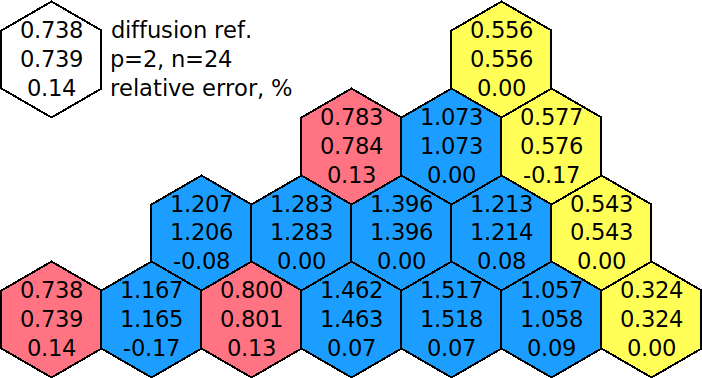
\includegraphics[width=0.85\linewidth]{diff_without_p2n24.png}\\
	\caption{Power and error distributions using diffusion model.}
	\label{fig:power_iaea_without_dif}
\end{center}
\end{figure}
\begin{figure}[htp]
\begin{center}
	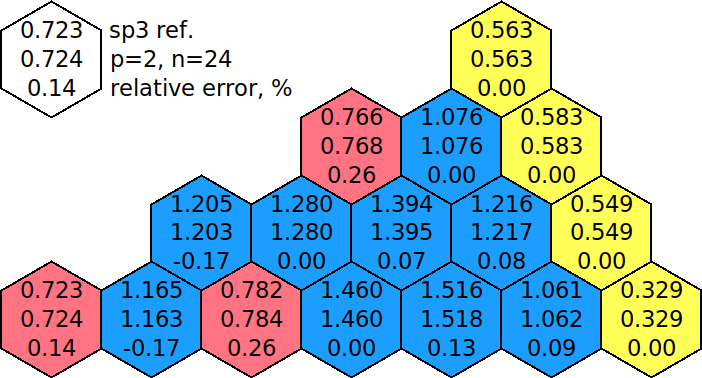
\includegraphics[width=0.85\linewidth]{sp3_without_p2n24.png}\\
	\caption{Power and error distributions using $\mathrm{SP_3}$ model.}
	\label{fig:power_ieae_without_sp3}
\end{center}
\end{figure}

\subsubsection{Solution of Alpha Modes spectral problem}
As a reference solution, the solutions obtained using the diffusion or transport model on a fine grid $ p = 3, n = 96 $ are taken.
Hereinafter, for $\alpha$-spectral problems, the following notation is used: $\alpha_{dif}$ --- $\alpha$-eigenvalue by diffusion model; $\alpha_{sp_3}$ --- $\alpha$-eigenvalue by $\mathrm{SP_3}$ model; $\Delta$ --- absolute deviation from the reference value.

\textbf{Without delayed neutrons.}

The results of solution of the $\alpha$-spectral problem without taking into account delayed neutrons using the different grids and finite elements are shown in Table~\ref{tab:iaea_without_alpha}.
These data demonstrate the convergence of approximate computed eigenvalues.

\begin{table}[htp]
\caption{The period eigenvalues.}
\label{tab:iaea_without_alpha}
\begin{center}
\begin{tabular}{c c r r r r}
\hline
$n$ & $p$ & $\alpha_{dif}$ & $\Delta_{dif}$ &$\alpha_{sp_3}$& $\Delta_{sp_3}$ \\
\hline
	& 1	& 556.3 & 100.8 & 532.7 & 104.1\\
6	& 2	& 465.6 & 10.1 & 440.0 & 11.4\\
	& 3	& 457.0 &  1.5 & 430.7 & 2.1\\ 
\hline
	& 1	& 488.1 & 32.6 & 463.0 & 34.4\\
24& 2	& 457.4 & 1.9 & 431.0 & 2.4\\
	& 3	& 455.7 & 0.2 & 428.9 & 0.3\\ 
\hline
	& 1	& 464.6 & 9.1 & 438.4 & 9.8\\
96& 2	& 455.8 & 0.3 & 428.9 & 0.3\\
	& 3	& 455.5 & -- & 428.6 & -- \\ 
\hline
Ref.& & 455.5 & & 428.6 \\ 
\hline
\end{tabular}
\end{center}
\end{table}

The results of solution of the spectral problem for the first 10 eigenvalues are shown in Table~\ref{tab:iaea_without_alpha_10}.
The eigenvalues $\lambda_1^{(\alpha)} \leq \lambda_2^{(\alpha)} \leq ...$ are well separated. 
In our example, the fundamental eigenvalue is less the rest and therefore the main harmonic  will attenuate more slowly than the rest.
A regular mode of the reactor is thereby defined.
The value $\alpha = \lambda_1^{(\alpha)}$ determines the amplitude of neutron field development and connects directly with reactor period in the regular mode.

\begin{table}[htp]
\caption{The eigenvalues $\alpha_i=\lambda_i^{(\alpha)}$ for $p=3, n=96$.}
\label{tab:iaea_without_alpha_10}
\begin{center}
\begin{tabular}{c r r}
\hline
$i$ & Diffusion & SP$_3$ \\
\hline
1 & 455.540 + 0.0$i$& 428.561 + 0.0$i$ \\
2 & 760.532 + 0.0$i$& 730.398 + 0.0$i$ \\
3 & 760.543 + 0.0$i$& 730.408 + 0.0$i$ \\
4 & 1267.192 + 0.0$i$&1228.835 + 0.0$i$ \\
5 & 1267.192 + 0.0$i$&1228.836 + 0.0$i$ \\
6 & 1647.145 + 0.0$i$&1601.437 + 0.0$i$ \\
7 & 2083.289 + 0.0$i$&2031.778 + 0.0$i$ \\
8 & 2696.887 + 0.0$i$&2616.862 + 0.0$i$ \\
9 & 3188.356 + 0.0$i$&3092.715 + 0.0$i$ \\
10& 3188.363 + 0.0$i$&3092.722 + 0.0$i$ \\
\hline
\end{tabular}
\end{center}
\end{table}

\begin{figure}[htp]
\begin{center}
	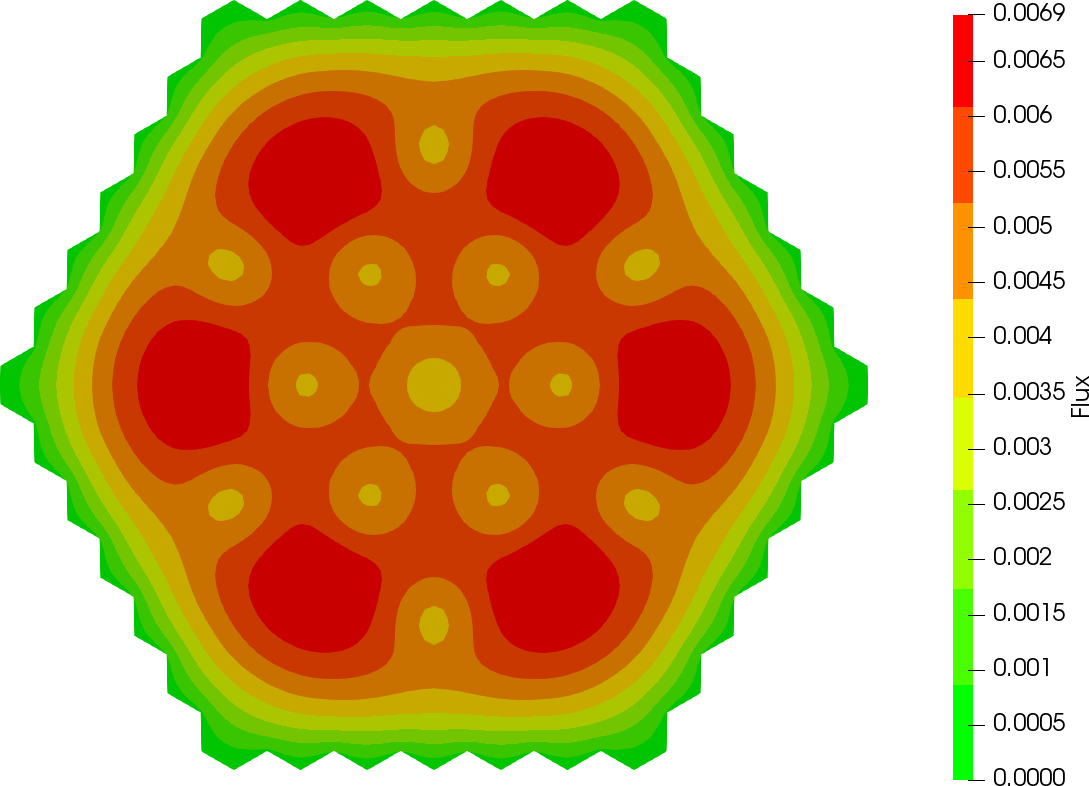
\includegraphics[width=0.49\linewidth]{iaea_without/alpha_sp3_u1_1_without.png}
	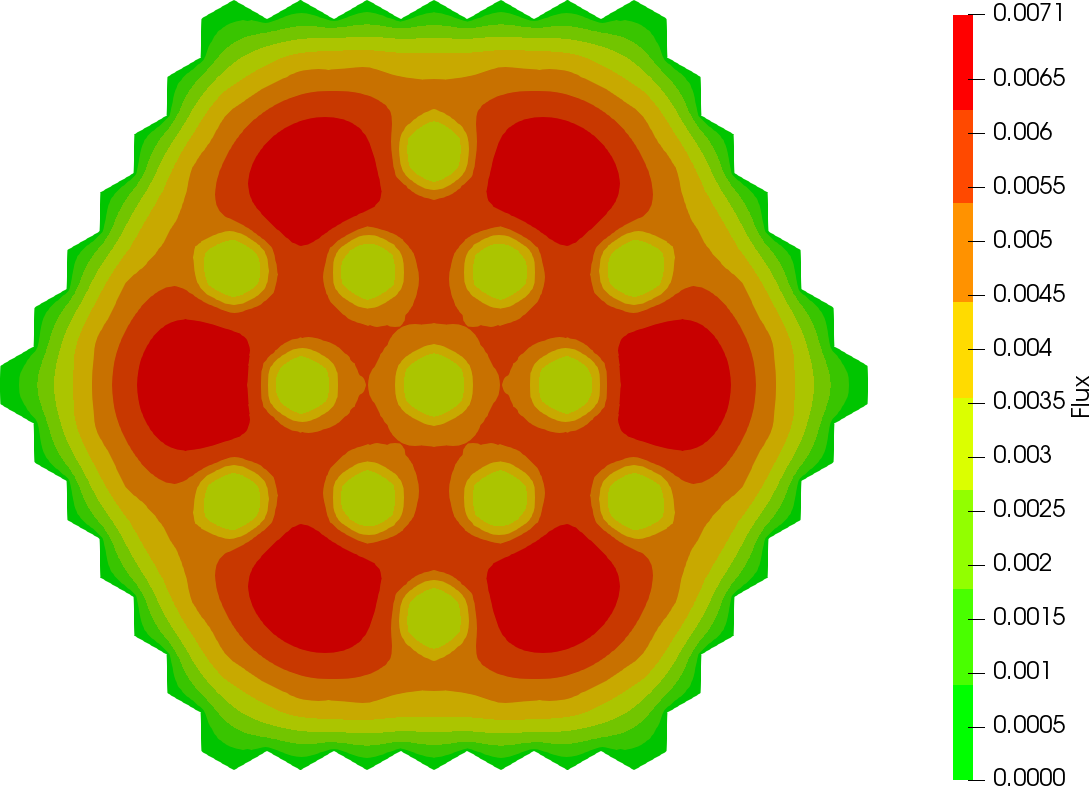
\includegraphics[width=0.49\linewidth]{iaea_without/alpha_sp3_u2_1_without.png}\\
	\caption{Eigenfunctions $\phi_1^{(1)}$, $\phi_2^{(1)}$ using $\mathrm{SP_3}$ model.}
	\label{fig:iaea_without_fun_1}
\end{center}
\end{figure}
\begin{figure}[htp]
\begin{center}
	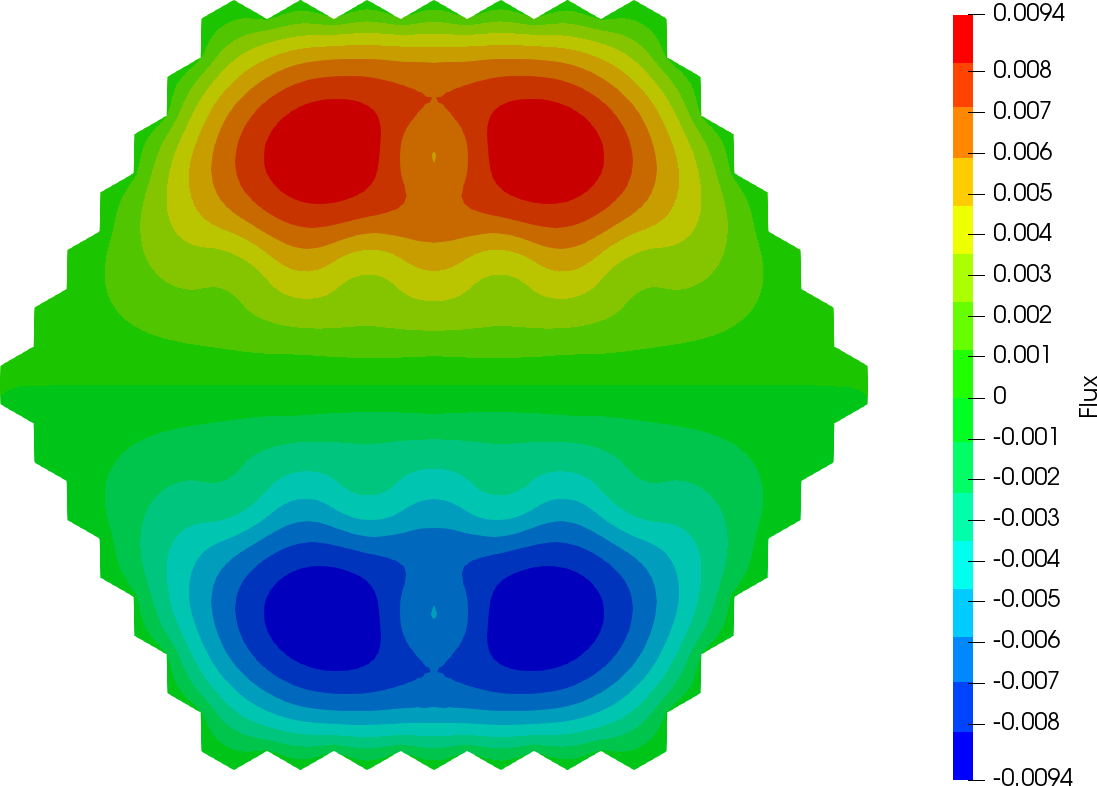
\includegraphics[width=0.49\linewidth]{iaea_without/alpha_sp3_u1_2_without.png}
	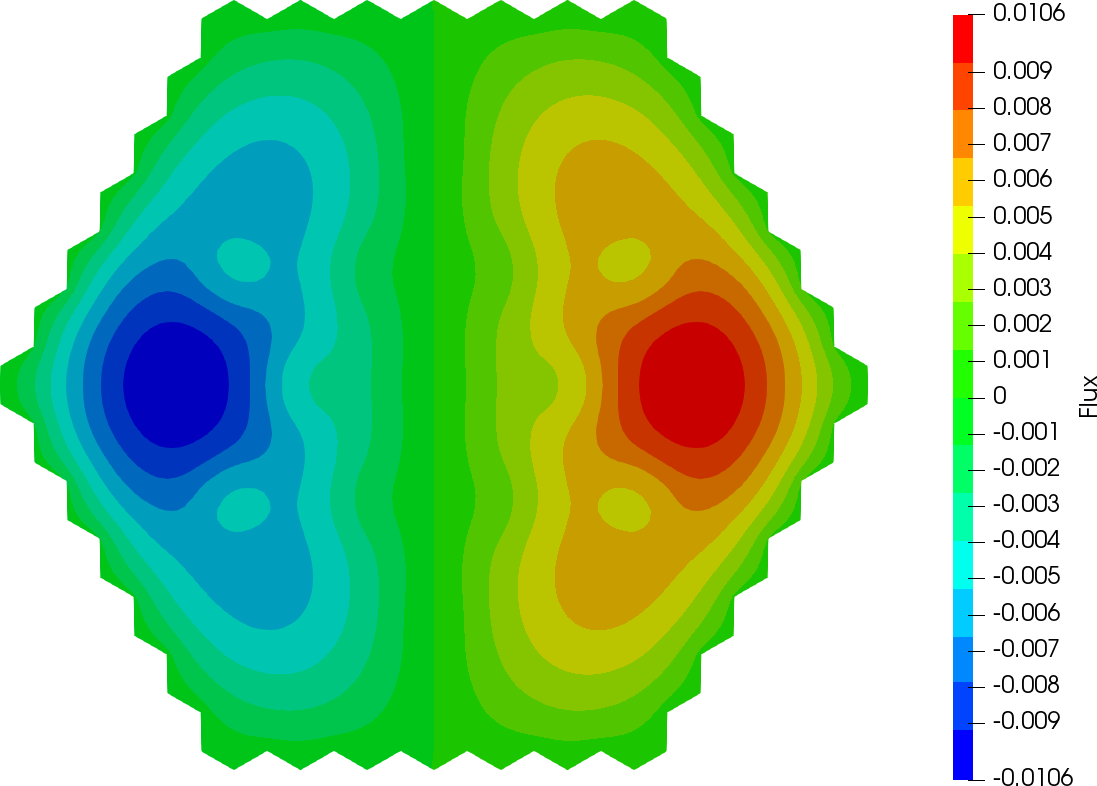
\includegraphics[width=0.49\linewidth]{iaea_without/alpha_sp3_u1_3_without.png}\\
	\caption{Eigenfunctions $\phi_1^{(2)}$, $\phi_1^{(3)}$ using $\mathrm{SP_3}$ model.}
	\label{fig:iaea_without_fun_2}
\end{center}
\end{figure}
\begin{figure}[htp]
\begin{center}
	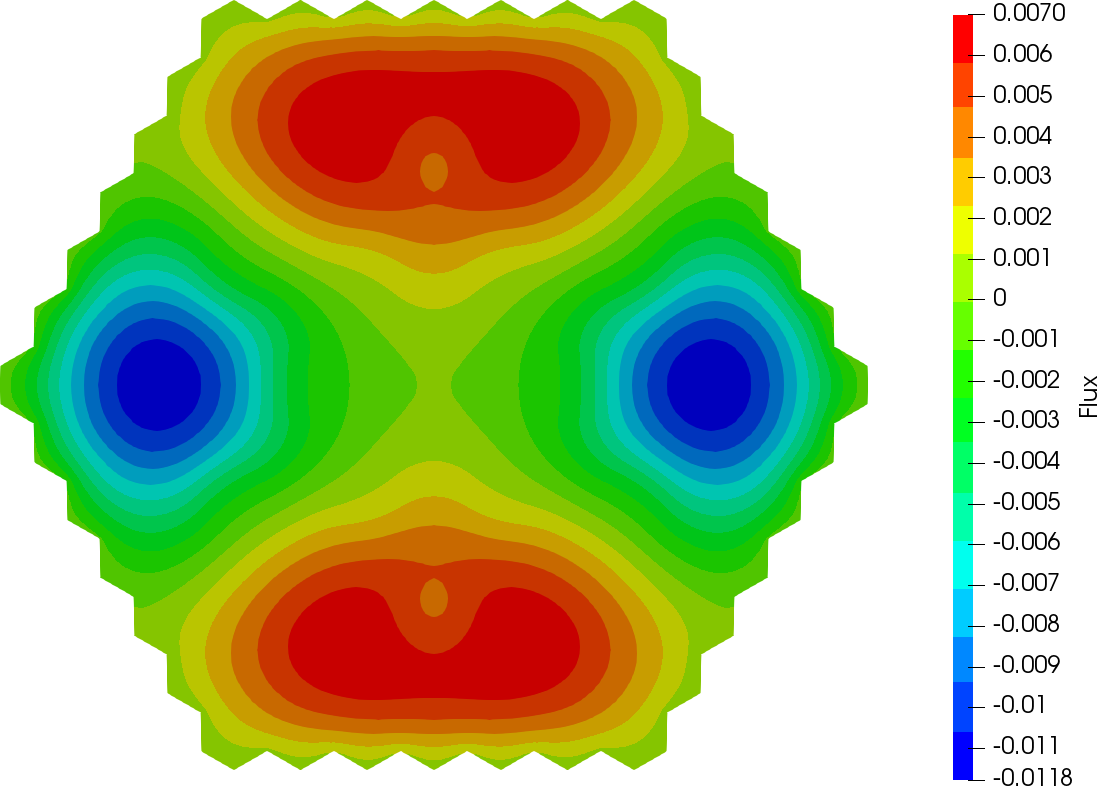
\includegraphics[width=0.49\linewidth]{iaea_without/alpha_sp3_u1_4_without.png}
	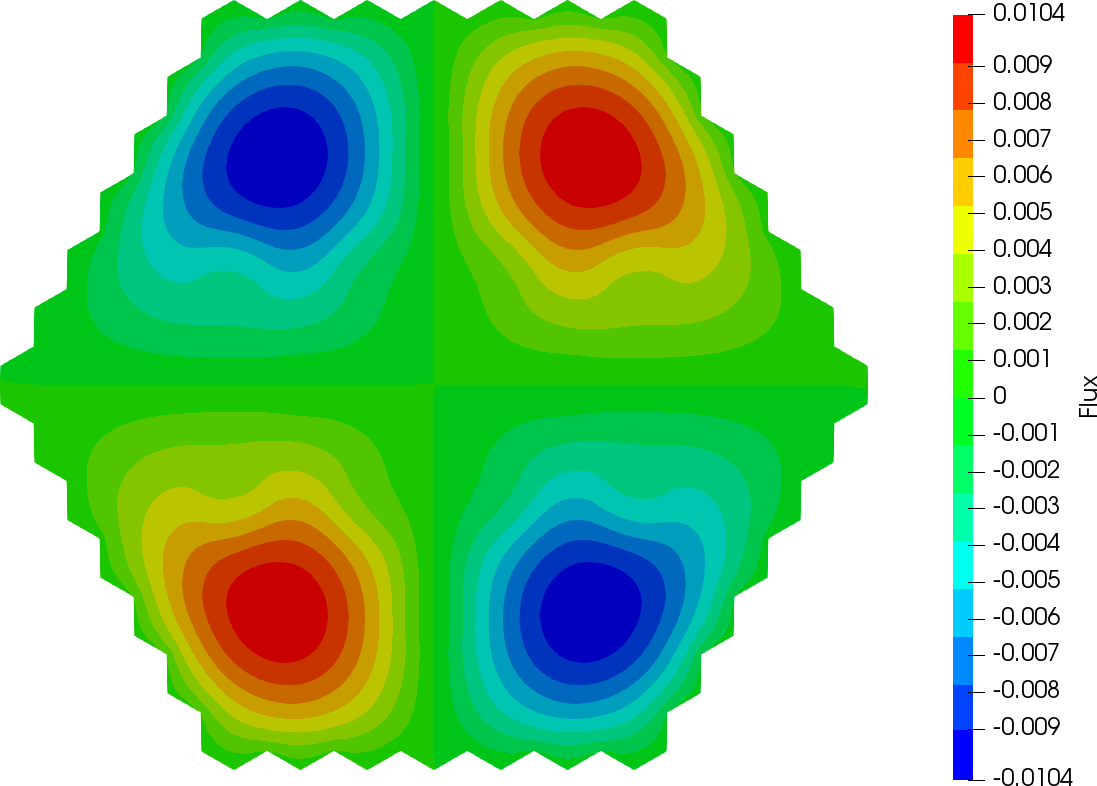
\includegraphics[width=0.49\linewidth]{iaea_without/alpha_sp3_u1_5_without.png}\\
	\caption{Eigenfunctions $\phi_1^{(4)}$, $\phi_1^{(5)}$ using $\mathrm{SP_3}$ model.}
	\label{fig:iaea_without_fun_3}
\end{center}
\end{figure}

The eigenfunctions for fundamental eigenvalue ($i=1$) of the $\alpha$-spectral problem without taking into account delayed neutron are shown in the Fig.~\ref{fig:iaea_without_fun_1}. 
Due to the fact that a state of the reactor is close to critical ($k=k_1\approx 0.97935$), the fundamental eigenfunctions of the $\lambda$-spectral problem are close to the fundamental eigenfunctions of the $\alpha$-spectral problem.
The eigenfunctions $\phi_1^{(i)}, i=2,3,4,5$ are shown in the Fig.~\ref{fig:iaea_without_fun_2}, Fig.~\ref{fig:iaea_without_fun_3}.

\textbf{With delayed neutrons.}

The results of solution of the $\alpha$-spectral problem taking into account delayed neutrons using the different grids and finite elements are shown in Table~\ref{tab:iaea_without_alpha_del}.
These data demonstrate the convergence of approximate computed eigenvalues.

\begin{table}[htp]
\caption{The period eigenvalues.}
\label{tab:iaea_without_alpha_del}
\begin{center}
\begin{tabular}{c c r r r r}
\hline
$n$ & $p$ & $\alpha_{dif}$ & $\Delta_{dif}$ &$\alpha_{sp_3}$& $\Delta_{sp_3}$ \\
\hline
	& 1	&0.06465 &0.00264&0.06410 & 0.00295\\
6	& 2	&0.06232 &0.00031&0.06153 & 0.00035\\
	& 3	&0.06206 &0.00005&0.06122 & 0.00007\\ 
\hline
	& 1	&0.06296 &0.00095&0.06224 & 0.00109\\
24& 2	&0.06207 &0.00005&0.06123 & 0.00008\\
	& 3	&0.06202 &0.00001&0.06116 & 0.00001\\ 
\hline
	& 1	&0.06228 &0.00027&0.06147 & 0.00032\\
96& 2	&0.06202 &0.00001&0.06116 & 0.00001\\
	& 3	&0.06201 &     --&0.06115 &      --\\ 
\hline
Ref.& & 0.06201 & & 0.06115 \\ 
\hline
\end{tabular}
\end{center}
\end{table}

The results of solution of the spectral problem for the first 10 eigenvalues are shown in Table~\ref{tab:iaea_without_alpha_del_10}.
Due to the contribution of delayed neutrons, the fundamental eigenvalue is much smaller than in the case without taking into account delayed neutrons.
Again the fundamental eigenvalue is less the rest and therefore the main harmonic  will attenuate more slowly than the rest.

\begin{table}[htp]
\caption{The eigenvalues $\alpha_i=\lambda_i^{(\alpha)}$ for $p=3, n=96$.}
\label{tab:iaea_without_alpha_del_10}
\begin{center}
\begin{tabular}{c r r}
\hline
$i$ & Diffusion & SP$_3$ \\
\hline
1& 0.06201 + 0.0$i$&0.06115 + 0.0$i$\\
2& 0.06837 + 0.0$i$&0.06796 + 0.0$i$\\
3& 0.06837 + 0.0$i$&0.06796 + 0.0$i$\\
4& 0.07279 + 0.0$i$&0.07258 + 0.0$i$\\
5& 0.07279 + 0.0$i$&0.07258 + 0.0$i$\\
6& 0.07446 + 0.0$i$&0.07430 + 0.0$i$\\
7& 0.07547 + 0.0$i$&0.07536 + 0.0$i$\\
8& 0.07662 + 0.0$i$&0.07652 + 0.0$i$\\
9& 0.07717 + 0.0$i$&0.07709 + 0.0$i$\\
10& 0.07721 + 0.0$i$&0.07711 + 0.0$i$\\
\hline
\end{tabular}
\end{center}
\end{table}

\begin{figure}[htp]
\begin{center}
	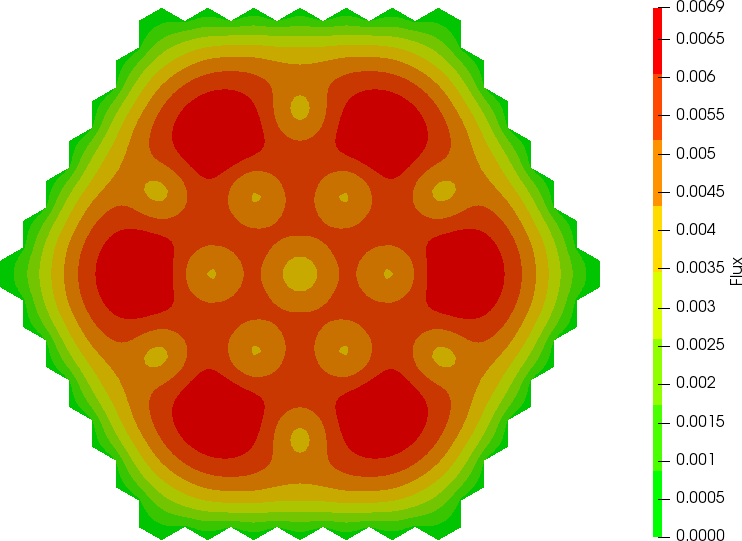
\includegraphics[width=0.49\linewidth]{iaea_without/alpha_delayed_sp3_u1_1_without.png}
	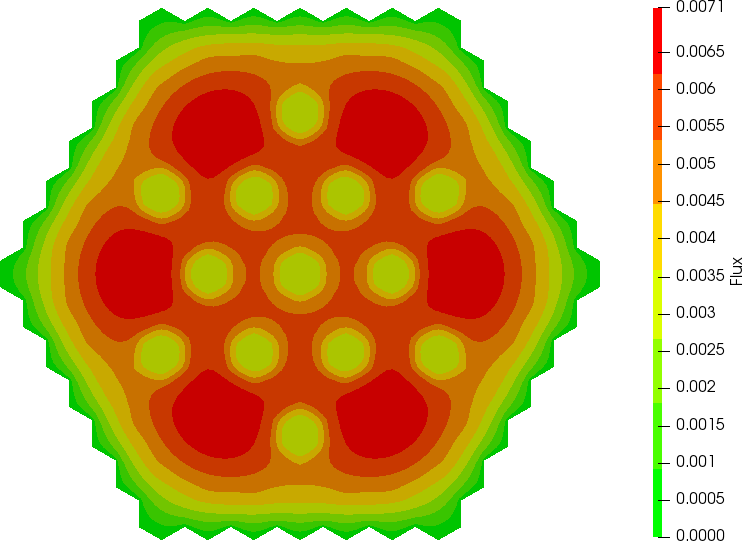
\includegraphics[width=0.49\linewidth]{iaea_without/alpha_delayed_sp3_u2_1_without.png}\\
	\caption{Eigenfunctions $\phi_1^{(1)}$, $\phi_2^{(1)}$.}
	\label{fig:iaea_without_fun_del_1}
\end{center}
\end{figure}
\begin{figure}[htp]
\begin{center}
	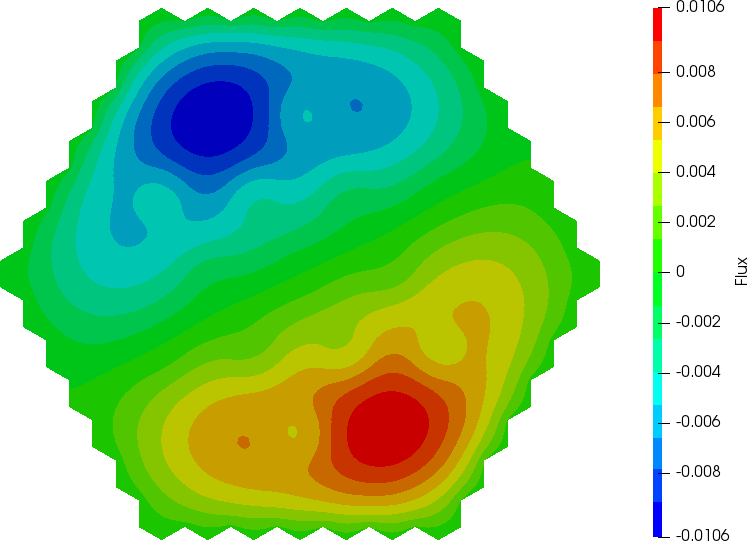
\includegraphics[width=0.49\linewidth]{iaea_without/alpha_delayed_sp3_u1_2_without.png}
	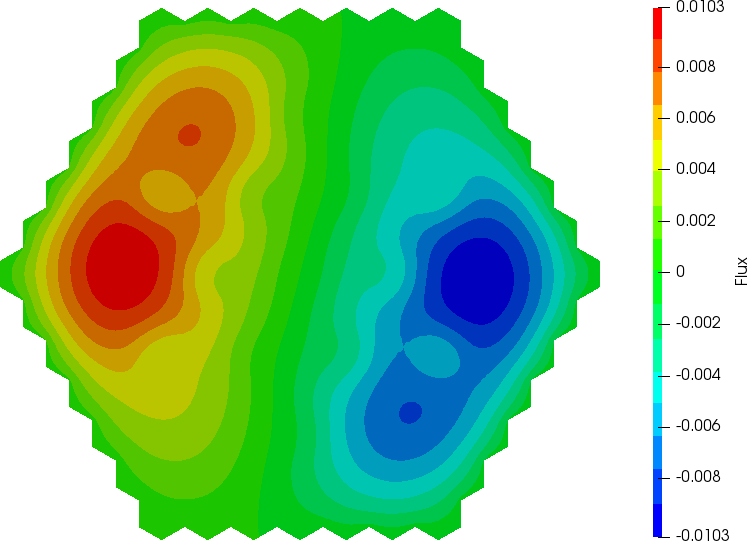
\includegraphics[width=0.49\linewidth]{iaea_without/alpha_delayed_sp3_u1_3_without.png}\\
	\caption{Eigenfunctions $\phi_1^{(2)}$, $\phi_1^{(3)}$.}
	\label{fig:iaea_without_fun_del_2}
\end{center}
\end{figure}
\begin{figure}[htp]
\begin{center}
	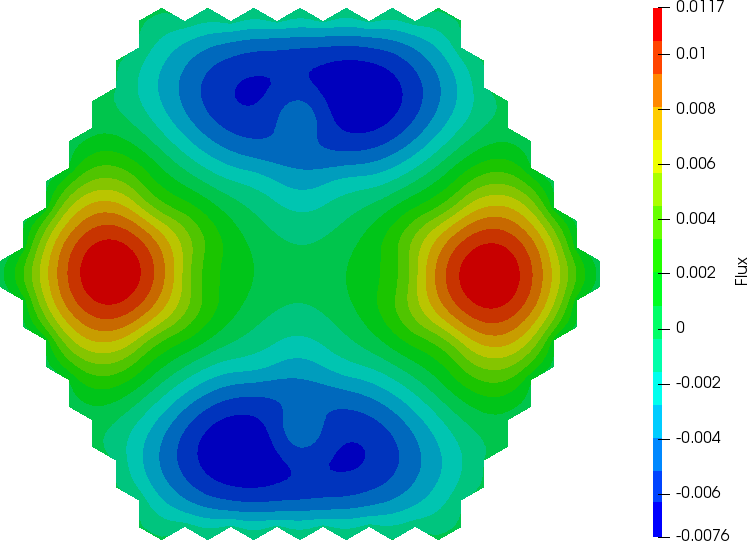
\includegraphics[width=0.49\linewidth]{iaea_without/alpha_delayed_sp3_u1_4_without.png}
	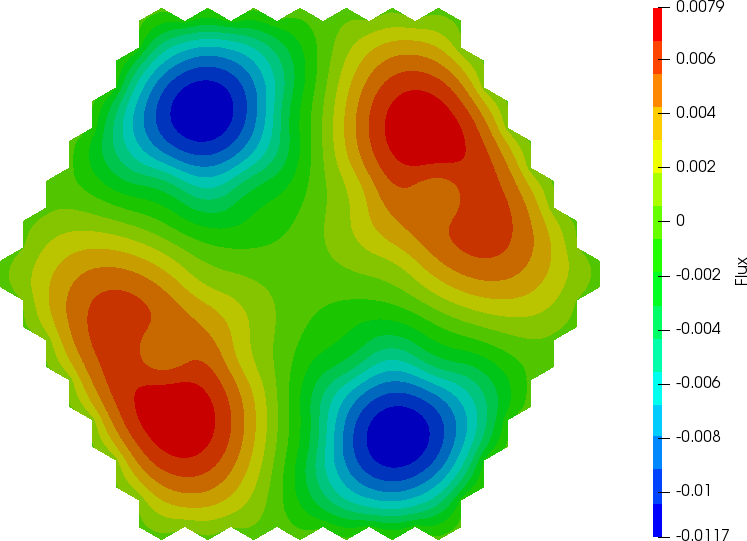
\includegraphics[width=0.49\linewidth]{iaea_without/alpha_delayed_sp3_u1_5_without.png}\\
	\caption{Eigenfunctions $\phi_1^{(4)}$, $\phi_1^{(5)}$.}
	\label{fig:iaea_without_fun_del_3}
\end{center}
\end{figure}

The eigenfunctions for fundamental eigenvalue ($i=1$) of the $\alpha$-spectral problem taking into account delayed neutron are shown in the Fig.~\ref{fig:iaea_without_fun_del_1}. 
The eigenfunctions $\phi_1^{(i)}, i=2,3,4,5$ are shown in the Fig.~\ref{fig:iaea_without_fun_del_2}, Fig.~\ref{fig:iaea_without_fun_del_3}.
The first eigenfunctions of the problems without taking into account and taking into account delayed neutrons are close to each other in topology.

\subsection{IAEA-2D with reflector}
Added external reflector row (material 4, see Table~\ref{tab:iaea}). 

\subsubsection{Solution of Lambda Modes spectral problem}
The obtained results by \citep{avvakumov2015} was taken as a reference solution for the diffusion model, and for the $\mathrm{SP_3}$ model ---  the solution obtained by MCNP4C code \citep{ryu2010development}.
The results of the solution of the effective multiplication factor for test IAEA-2D with a reflector are shown in Table~\ref{tab:iaea_with_lambda}. 

\begin{table}[htp]
\caption{The effective multiplication factor.}
\label{tab:iaea_with_lambda}
\begin{center}
\begin{tabular}{c c r r r r r r}
\hline
$n$ & $p$ & $k_{dif}$ & $\Delta_{dif}$ & $\delta_{dif}$ &$k_{sp_3}$& $\Delta_{sp_3}$ & $\delta_{sp_3}$ \\
\hline
	& 1	& 1.01041& 490&13.29& 1.01159& 536& 14.14\\
6	& 2	& 1.00623&  72& 1.88& 1.00711&  88&  2.19\\
	& 3	& 1.00558&   7& 0.22& 1.00636&  13&  0.35\\ 
\hline
	& 1	& 1.00699& 148& 4.54& 1.00792& 169&  4.96\\
24& 2	& 1.00561&  10& 0.30& 1.00640&  17&  0.42\\
	& 3	& 1.00551&   0& 0.02& 1.00626&   3&  0.17\\ 
\hline
	& 1	& 1.00591&  36& 1.28& 1.00671&  48&  1.42\\
96& 2	& 1.00552&   1& 0.04& 1.00626&   3&  0.18\\
	& 3	& 1.00551&   0& 0.01& 1.00625&   2&  0.18\\ 
\hline
Ref.&   & 1.00551&    &     & 1.00623&     &\\ 
\hline
\end{tabular}
\end{center}
\end{table}

\begin{table}[h]
\caption{The eigenvalues $k_i=1/\lambda_i^{(k)}$ for $p=3, n=96$.}
\label{tab:iaea_with_lambda_10}
\begin{center}
\begin{tabular}{c r r}
\hline
$i$ & Diffusion & SP$_3$  \\
\hline
1 & 1.00551 + 0.0$i$ & 1.00625 + 0.0$i$\\
2 & 0.99649 + 0.0$i$ & 0.99725 + 0.0$i$\\
3 & 0.99649 + 0.0$i$ & 0.99725 + 0.0$i$\\
4 & 0.97679 + 0.0$i$ & 0.97776 + 0.0$i$\\
5 & 0.97679 + 0.0$i$ & 0.97776 + 0.0$i$\\
6 & 0.95868 + 0.0$i$ & 0.95990 + 0.0$i$\\
7 & 0.92898 + 0.0$i$ & 0.93097 + 0.0$i$\\
8 & 0.92419 + 0.0$i$ & 0.92593 + 0.0$i$\\
9 & 0.90479 + 0.0$i$ & 0.90735 + 0.0$i$\\
10 & 0.90479 + 0.0$i$ & 0.90735 + 0.0$i$\\
\hline
\end{tabular}
\end{center}
\end{table}

\begin{figure}[h]
\begin{center}
	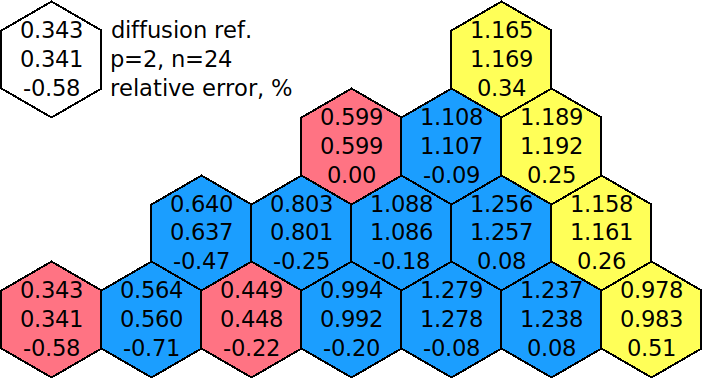
\includegraphics[width=0.85\linewidth]{diff_p2n24.png}\\
	\caption{Power and error distributions using diffusion model.}
	\label{fig:power_iaea_with_dif}
\end{center}
\end{figure}

\begin{figure}[h]
\begin{center}
	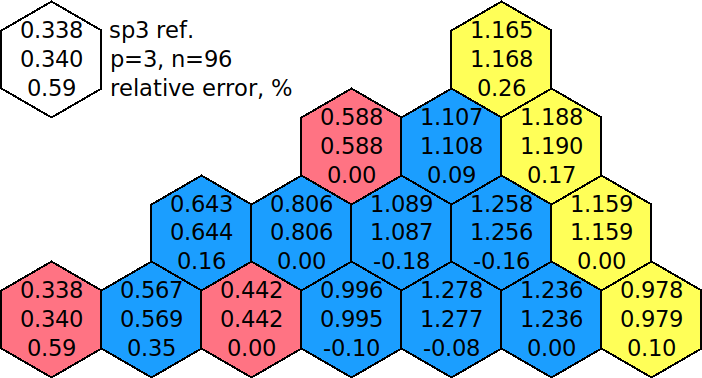
\includegraphics[width=0.85\linewidth]{sp3_p3n96.png}\\
	\caption{Power and error distributions using $\mathrm{SP_3}$ model.}
	\label{fig:power_iaea_with_sp3}
\end{center}
\end{figure}

The results of the first 10 eigenvalues for $ p = 3, n = 96 $ is shown in Table~\ref{tab:iaea_with_lambda_10}.
The power and error distribution for $p = 2, n = 24$ using diffusion model is shown in the Fig~\ref{fig:power_iaea_with_dif} and for $p = 3, n = 96$ using $\mathrm{SP_3}$ model is shown Fig~\ref{fig:power_iaea_with_sp3}.

%В таблице \ref{tab:iaea_with_lambda_10} приведены результаты первых 10 собственных значений при $p=3, n=96$.
%Распределение мощности при $p=2, n=24$ по диффузионной и при $p=3, n=96$ по SP$_3$ моделях показаны на рисунках \ref{ris:power1}, \ref{ris:power2}  соответственно.

\subsubsection{Solution of Alpha Modes spectral problem}
As a reference solution, the solutions obtained using the diffusion or transport model on a fine grid $ p = 3, n = 96 $ are taken.
 
\textbf{Without delayed neutrons.}

%В таблице \ref{tab:iaea_with_alpha} показаны результаты расчета $\alpha$-спектральной задачи без учета запаздывающих нейтронов при использовании различных сеток и конечных элементов. Эти данные демонстрируют сходимость приближенно вычисляемых собственных значений при сгущении сетки $n$ и при увеличении степени аппроксимирующих полиномов $p$. 
%В таблице \ref{tab:iaea_with_alpha_10} приведены результаты первых десяти собственных значений $\alpha$-спектральной задачи (\ref{1.10}) при мелкой сетке $p=3, n=96$. 
%Сами собственные значения   $\mathrm{Re}\lambda_1^{(\alpha)} \leq \mathrm{Re}\lambda_2^{(\alpha)} \leq ...$ хорошо отделены друг от друга.
%В нашем примере главное собственное значение отрицательное и поэтому главная гармоника будет возрастать, а все остальные затухать.
%На рисунках \ref{fig:iaea_with_fun_1}, \ref{fig:iaea_with_fun_2}, \ref{fig:iaea_with_fun_3} показаны собственные функции для SP$_3$ модели.

\begin{table}[h]
\caption{The period eigenvalues.}
\label{tab:iaea_with_alpha}
\begin{center}
\begin{tabular}{c c r r r r}
\hline
$n$ & $p$ & $\alpha_{dif}$ & $\Delta_{dif}$ &$\alpha_{sp_3}$& $\Delta_{sp_3}$ \\
\hline
	& 1	& $-$184.95 & 84.14 & $-$205.92 & 91.32\\
6	& 2	& $-$113.58 & 12.77 & $-$130.02 & 15.42\\
	& 3	& $-$101.98 &  1.17 & $-$116.72 &  2.12\\ 
\hline
	& 1	& $-$126.66 & 25.85 & $-$143.85 & 29.25\\
24& 2	& $-$102.58 &  1.77 & $-$117.31 &  2.71\\
	& 3	& $-$100.88 &  0.07 & $-$114.83 &  0.23\\ 
\hline
	& 1	& $-$107.82 &  7.01 & $-$122.84 & 8.24\\
96& 2	& $-$100.97 &  0.16 & $-$114.94 & 0.34\\
	& 3	& $-$100.81 &	 -- & $-$114.60 &  -- \\ 
\hline
Ref.& & $-$100.81 & & $-$114.60 \\ 
\hline
\end{tabular}
\end{center}
\end{table}

\begin{table}[h]
\caption{The eigenvalues $\alpha_i=\lambda_i^{(\alpha)}$ for $p=3, n=96$.}
\label{tab:iaea_with_alpha_10}
\begin{center}
\begin{tabular}{c r r}
\hline
$i$ & Diffusion & SP$_3$ \\
\hline
1 &$-$100.81 + 0.0$i$&$-$114.60 + 0.0$i$ \\
2 &  62.93 + 0.0$i$& 49.42 + 0.0$i$ \\
3 &  62.93 + 0.0$i$& 49.42 + 0.0$i$ \\
4 & 405.31 + 0.0$i$&390.15 + 0.0$i$ \\
5 & 405.31 + 0.0$i$&390.15 + 0.0$i$ \\
6 & 710.64 + 0.0$i$&693.47 + 0.0$i$ \\
7 &1141.43 + 0.0$i$&1118.67 + 0.0$i$ \\
8 &1469.68 + 0.0$i$&1438.31 + 0.0$i$ \\
9 &1494.37 + 0.0$i$&1468.54 + 0.0$i$ \\
10&1494.37 + 0.0$i$&1468.54 + 0.0$i$ \\
\hline
\end{tabular}
\end{center}
\end{table}

\begin{figure}[h]
\begin{center}
	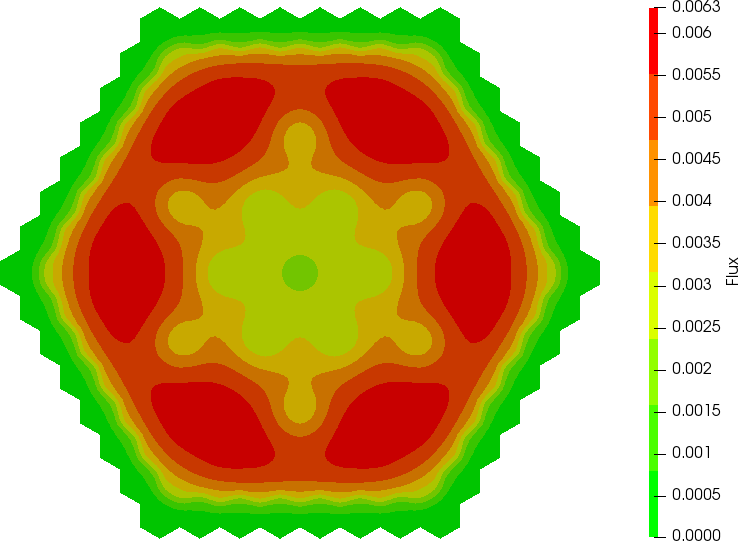
\includegraphics[width=0.49\linewidth]{iaea_with/alpha_sp3_u1_1.png}
	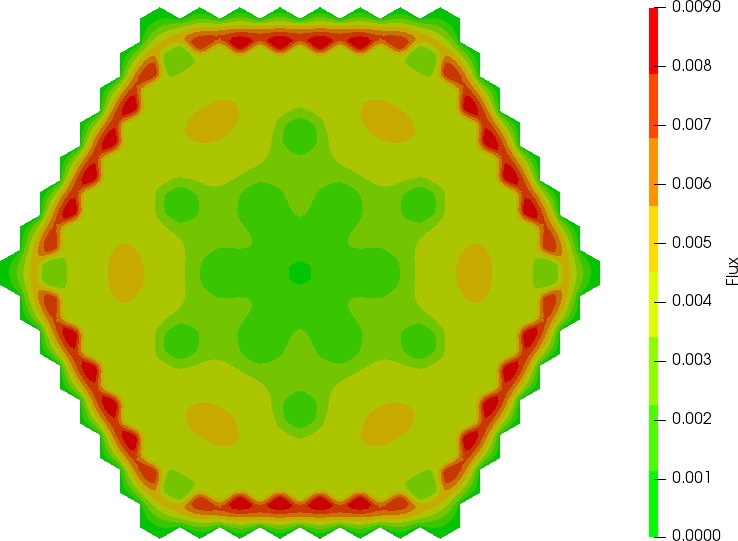
\includegraphics[width=0.49\linewidth]{iaea_with/alpha_sp3_u2_1.png}\\
	\caption{Eigenfuncions $\phi_1^{(1)}$, $\phi_2^{(1)}$.}
	\label{fig:iaea_with_fun_1}
\end{center}
\end{figure}

\begin{figure}[h]
\begin{center}
	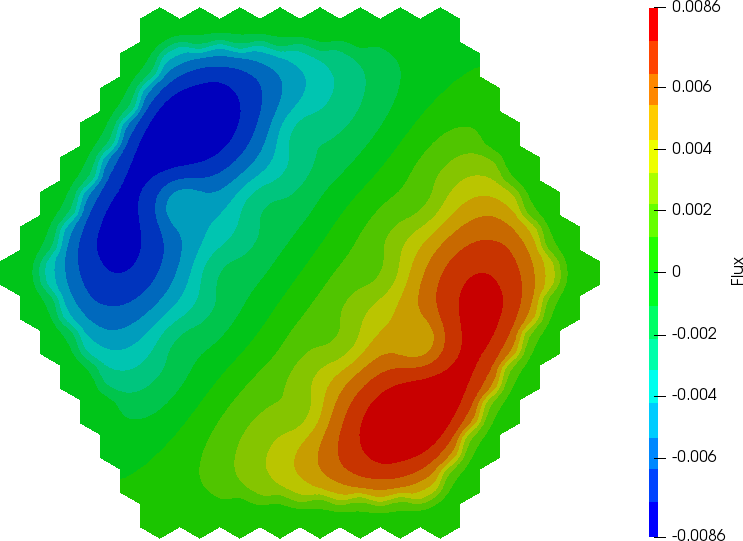
\includegraphics[width=0.49\linewidth]{iaea_with/alpha_sp3_u1_2.png}
	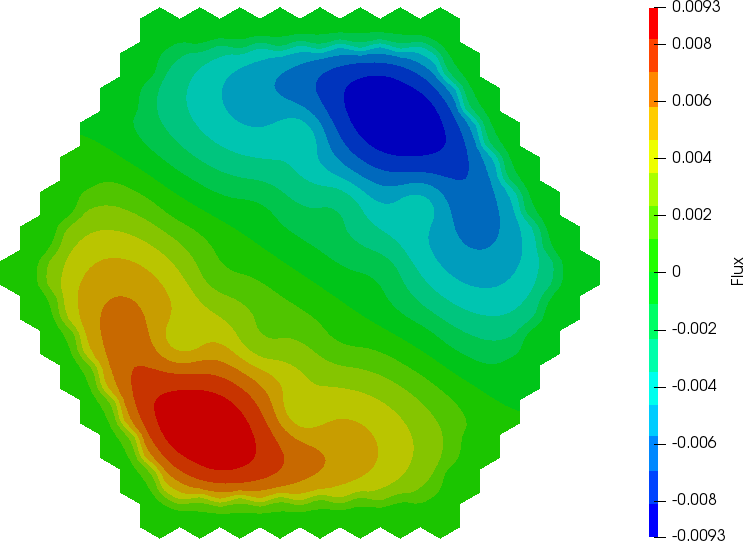
\includegraphics[width=0.49\linewidth]{iaea_with/alpha_sp3_u1_3.png}\\
	\caption{Eigenfuncions $\phi_1^{(2)}$, $\phi_1^{(3)}$.}
	\label{fig:iaea_with_fun_2}
\end{center}
\end{figure}

\begin{figure}[h]
\begin{center}
	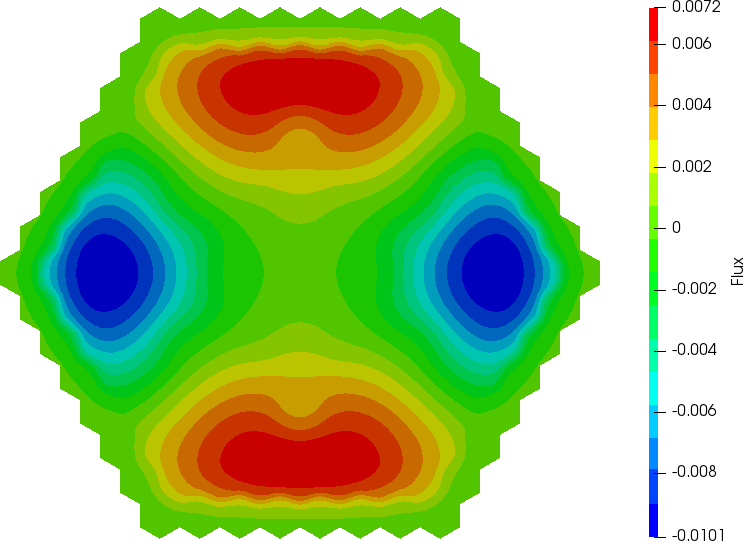
\includegraphics[width=0.49\linewidth]{iaea_with/alpha_sp3_u1_4.png}
	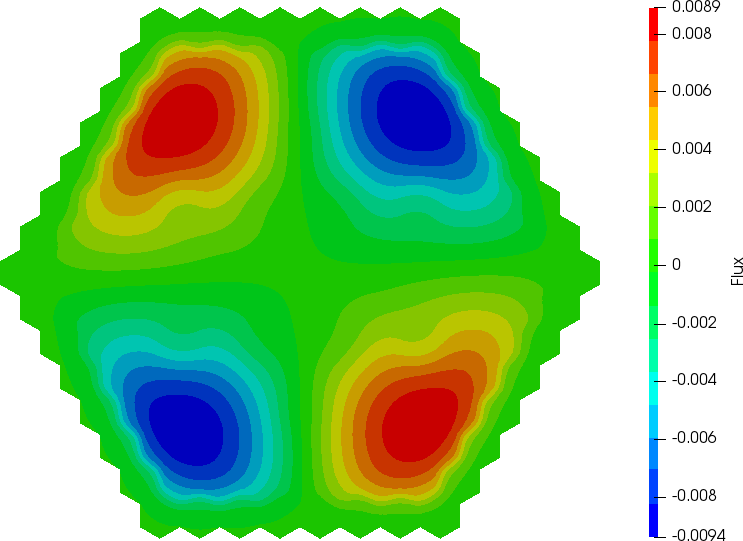
\includegraphics[width=0.49\linewidth]{iaea_with/alpha_sp3_u1_5.png}\\
	\caption{Eigenfuncions $\phi_1^{(4)}$, $\phi_1^{(5)}$.}
	\label{fig:iaea_with_fun_3}
\end{center}
\end{figure}

\textbf{With delayed neutrons.}

%В таблице \ref{tab:iaea_with_alpha_del} показаны результаты расчета $\alpha$-спектральной задачи с учетом запаздывающих нейтронов при использовании различных сеток и конечных элементов. Эти данные демонстрируют сходимость приближенно вычисляемых собственных значений при сгущении сетки $n$ и при увеличении степени аппроксимирующих полиномов $p$. 
%В таблице \ref{tab:iaea_with_alpha_del} приведены результаты первых десяти собственных значений $\alpha$-спектральной задачи (\ref{1.9}).
%Из-за вклада запаздывающих нейтронов главное собственное значение намного меньше, чем в случае без учета запаздывающих нейтронов.
%Снова главное собственное значение отрицательно и поэтому главная гармоника будет нарастать, а все остальные затухать.
%На рисунках \ref{ris:eigen4}, \ref{ris:eigen5}, \ref{ris:eigen6} показаны собственные функции для SP$_3$ модели.

\begin{table}[h]
\caption{The period eigenvalues.}
\label{tab:iaea_with_alpha_del}
\begin{center}
\begin{tabular}{c c r r r r}
\hline
$n$ & $p$ & $\alpha_{dif}$ & $\Delta_{dif}$ &$\alpha_{sp_3}$& $\Delta_{sp_3}$ \\
\hline
	& 1	&$-$68.2268 &67.8084& $-$88.9461 &87.6086\\
6	& 2	& $-$1.2810 & 0.8626& $-$11.1554 & 9.8179\\
	& 3	& $-$0.4506 & 0.0322&  $-$1.8063 & 0.4688\\ 
\hline
	& 1	& $-$9.0267  & 8.6083&$-$25.1658 &23.8283\\
24& 2	& $-$0.4686  & 0.0502& $-$1.9832 & 0.6457\\
	& 3	& $-$0.4202  & 0.0018& $-$1.3787 & 0.0412\\ 
\hline
	& 1	& $-$0.7018  & 0.2834& $-$4.9794 & 3.6419\\
96& 2	& $-$0.4225  & 0.0041& $-$1.3994 & 0.0619\\
	& 3	& $-$0.4184  &    -- & $-$1.3375 &    --\\ 
\hline
Ref.& & $-$0.4184 & & $-$1.3375 \\ 
\hline
\end{tabular}
\end{center}
\end{table}

\begin{table}[h]
\caption{The eigenvalues $\alpha_i=\lambda_i^{(\alpha)}$ for $p=3, n=96$.}
\label{tab:iaea_with_alpha_del_10}
\begin{center}
\begin{tabular}{c r r}
\hline
$i$ & Diffusion & SP$_3$ \\
\hline
1& $-$0.4184 + 0.0$i$&$-$1.3374 + 0.0$i$\\
2& 0.0281 + 0.0$i$&0.0238 + 0.0$i$\\
3& 0.0281 + 0.0$i$&0.0238 + 0.0$i$\\
4& 0.0628 + 0.0$i$&0.0622 + 0.0$i$\\
5& 0.0628 + 0.0$i$&0.0622 + 0.0$i$\\
6& 0.0695 + 0.0$i$&0.0692 + 0.0$i$\\
7& 0.0737 + 0.0$i$&0.0736 + 0.0$i$\\
8& 0.0741 + 0.0$i$&0.0740 + 0.0$i$\\
9& 0.0754 + 0.0$i$&0.0752 + 0.0$i$\\
10& 0.0763 + 0.0$i$&0.0762 + 0.0$i$\\
\hline
\end{tabular}
\end{center}
\end{table}

\begin{figure}[h]
\begin{center}
	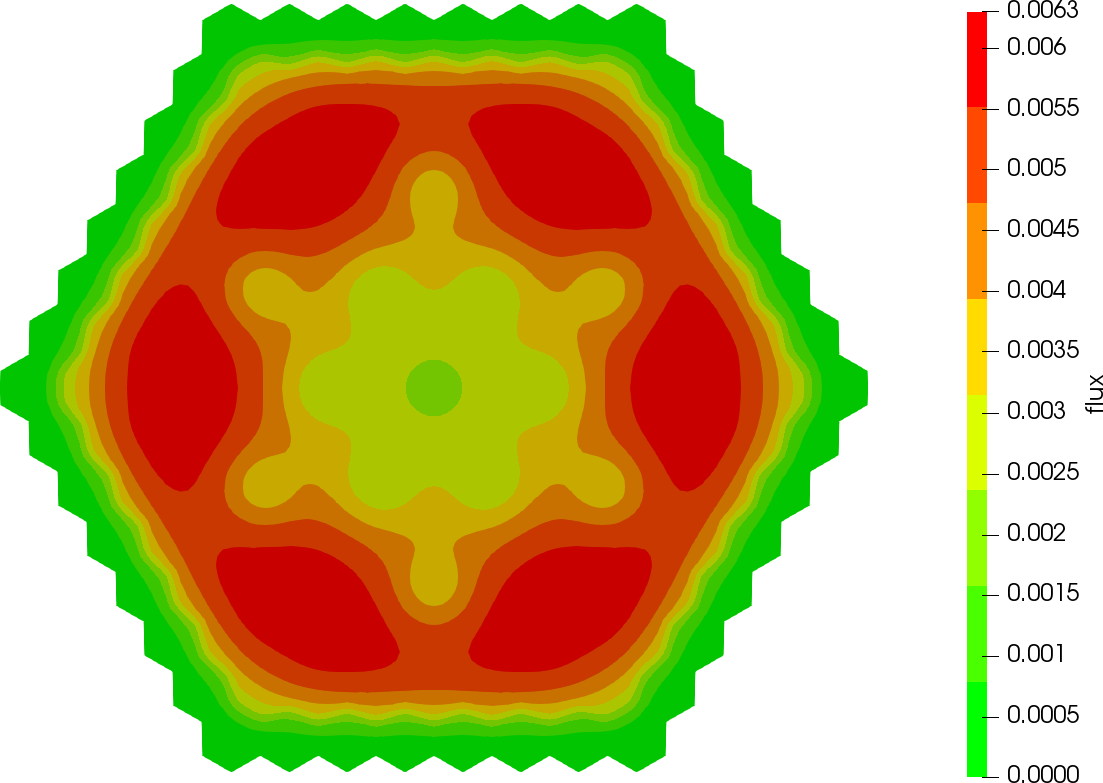
\includegraphics[width=0.49\linewidth]{iaea_with/alpha_delayed_sp3_u1_1.png}
	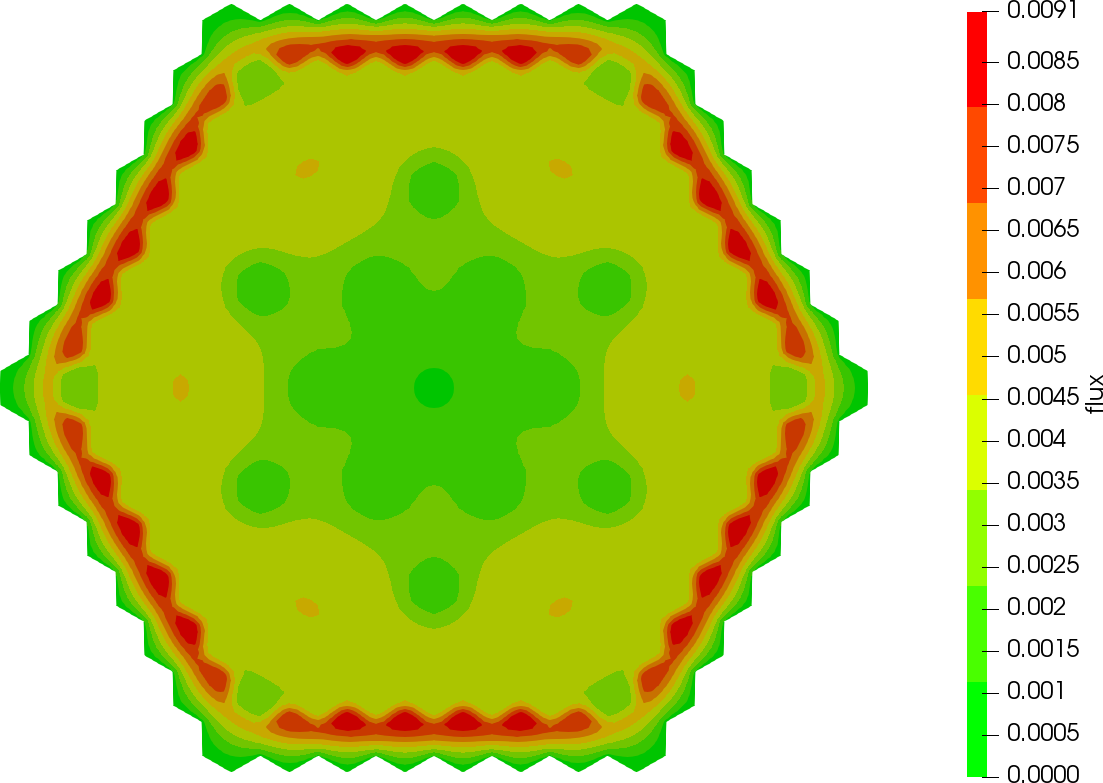
\includegraphics[width=0.49\linewidth]{iaea_with/alpha_delayed_sp3_u2_1.png}\\
	\caption{Eigenfunctions $\phi_1^{(1)}$, $\phi_2^{(1)}$.}
	\label{fig:iaea_with_fun_del_1}
\end{center}
\end{figure}

\begin{figure}[h]
\begin{center}
	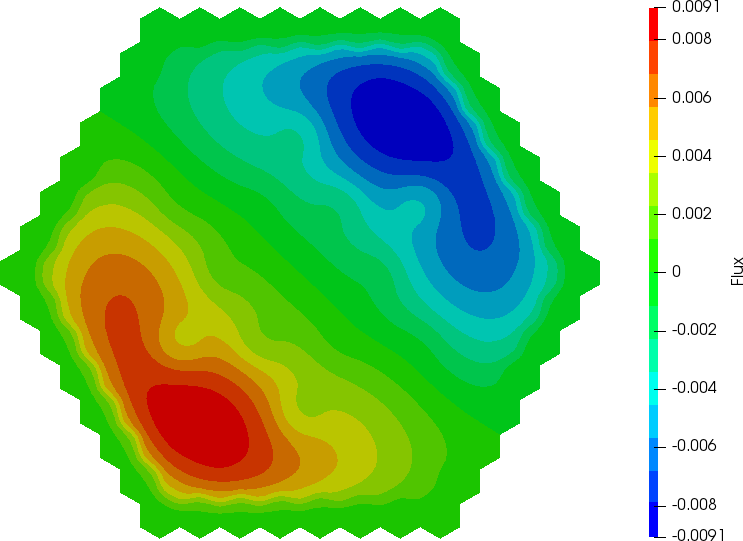
\includegraphics[width=0.49\linewidth]{iaea_with/alpha_delayed_sp3_u1_2.png}
	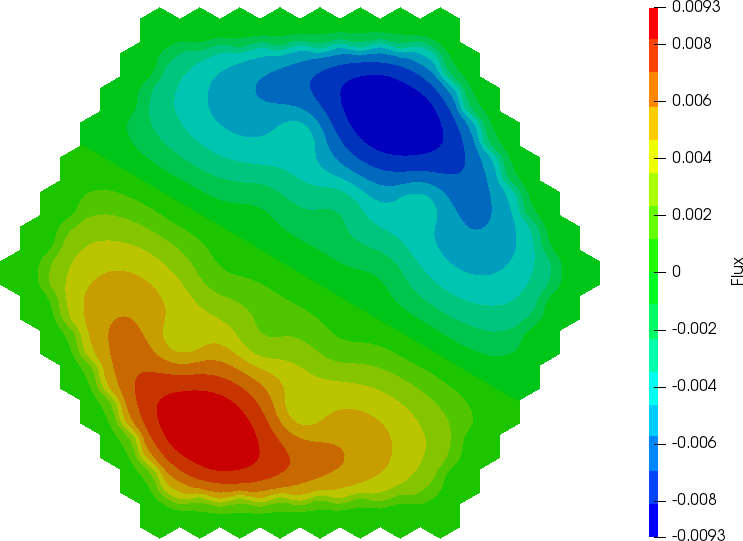
\includegraphics[width=0.49\linewidth]{iaea_with/alpha_delayed_sp3_u1_3.png}\\
	\caption{Eigenfunctions $\phi_1^{(2)}$, $\phi_1^{(3)}$.}
	\label{fig:iaea_with_fun_del_2}
\end{center}
\end{figure}

\begin{figure}[h]
\begin{center}
	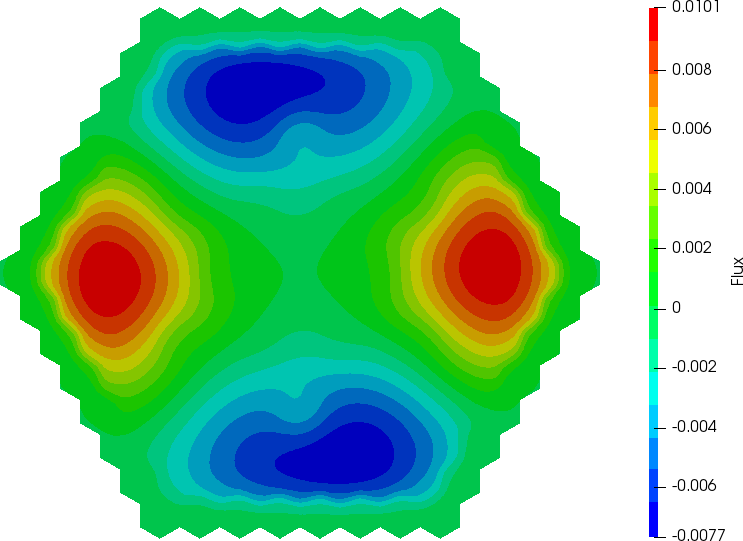
\includegraphics[width=0.49\linewidth]{iaea_with/alpha_delayed_sp3_u1_4.png}
	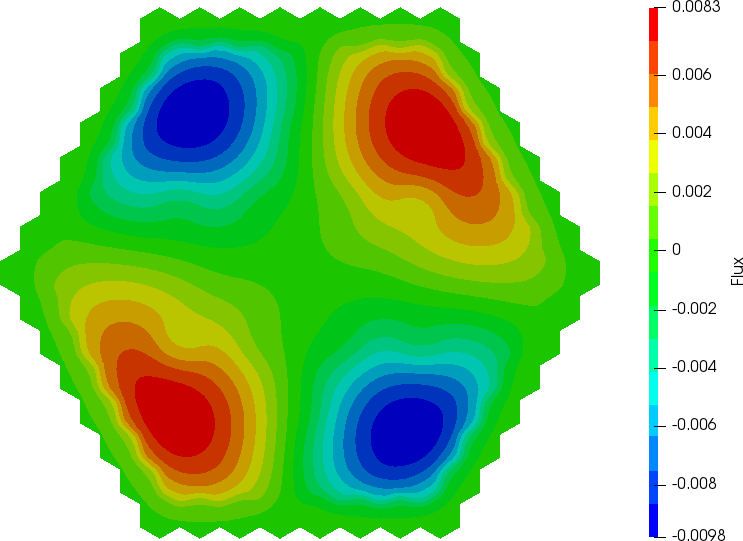
\includegraphics[width=0.49\linewidth]{iaea_with/alpha_delayed_sp3_u1_5.png}\\
	\caption{Eigenfunctions $\phi_1^{(4)}$, $\phi_1^{(5)}$.}
	\label{fig:iaea_with_fun_del_3}
\end{center}
\end{figure}

\subsection{Cosymmetric IAEA-2D with reflector}
Two rods added.
The geometrical model of reactor core is shown in Fig. \ref{fig:iaea_cosym}. 

\begin{figure}[h]
\begin{center}
	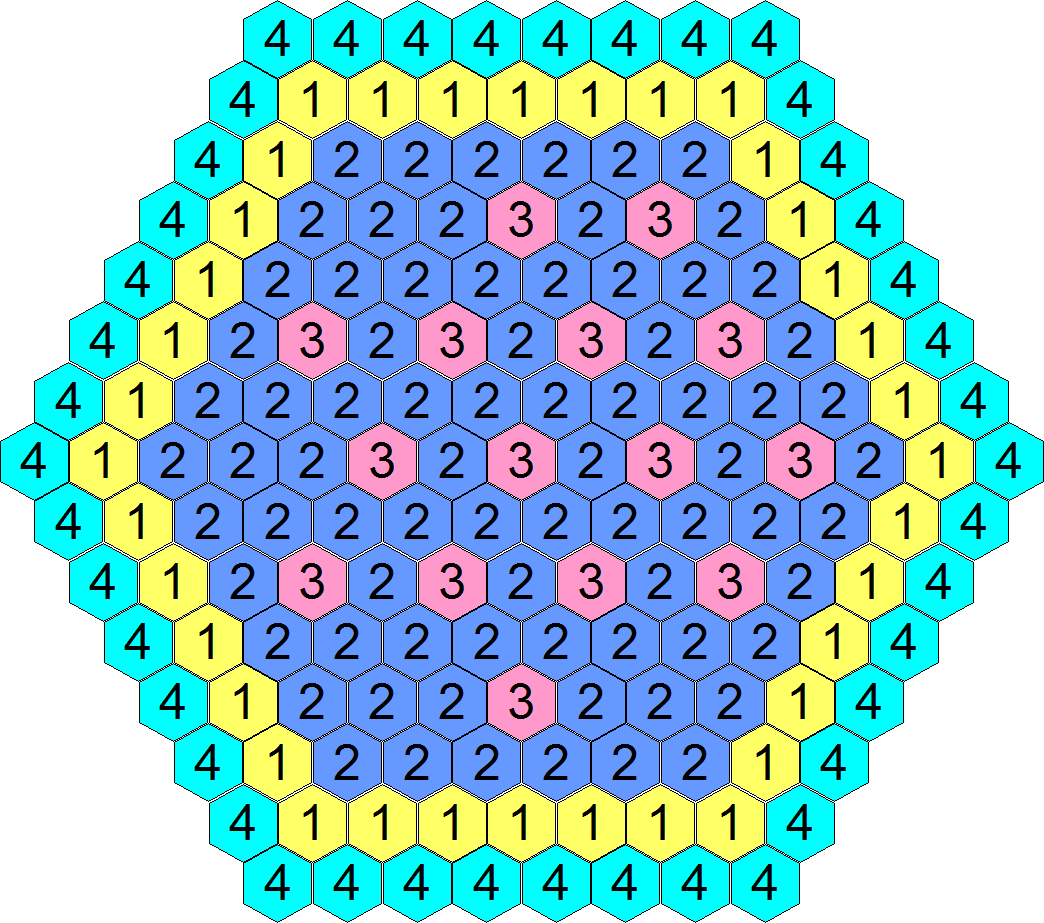
\includegraphics[width=0.6\linewidth]{iaea_cosym.png}\\
	\caption{Geometrcial model of the cosymmetric IAEA-2D reactor core with reflector.}
	\label{fig:iaea_cosym}
\end{center}
\end{figure}

\subsubsection{Solution of Lambda Modes spectral problem}
%В качестве эталонного решения взяты решение на мелкой сетке при $p=3, n=96$ по соответствующей модели.
%Результаты расчета кососимметричного теста IAEA-2D с отражателем приведены в таблице \ref{tab:iaea_cosym_lambda}. 
%В таблице \ref{tab:iaea_cosym_lambda_10} приведены результаты первых 10 собственных значений при $p=3, n=96$. 

\begin{table}[h]
\caption{The effective multiplication factor.}
\label{tab:iaea_cosym_lambda}
\begin{center}
\begin{tabular}{r r r r r r}
\hline
$n$ & $p$ & $k_{dif}$ & $\Delta_{dif}$ &$k_{sp_3}$& $\Delta_{sp_3}$ \\
\hline
	& 1	& 1.00809& 509& 1.00931& 556\\
6	& 2	& 1.00374&  74& 1.00465&  90\\
	& 3	& 1.00306&   6& 1.00387&  12\\
\hline
	& 1	& 1.00454& 154& 1.00550& 175\\
24& 2	& 1.00310&  10& 1.00391&  16\\
	& 3	& 1.00300&   0& 1.00376&   1\\ 
\hline
	& 1	& 1.00341&  41& 1.00424&  49\\
96& 2	& 1.00300&   0& 1.00377&   2\\
	& 3	& 1.00300&  --& 1.00375&  --\\ 
\hline
Ref.&   & 1.00300&    & 1.00375&    \\ 
\hline
\end{tabular}
\end{center}
\end{table}

\begin{table}[h]
\caption{The eigenvalues $k_i=1/\lambda_i^{(k)}$ for $p=3, n=96$.}
\label{tab:iaea_cosym_lambda_10}
\begin{center}
\begin{tabular}{rrr}
\hline
$i$ & diffusion & SP$_3$  \\
\hline
1 & 1.00300 + 0.0$i$ & 1.00375 + 0.0$i$\\
2 & 0.99457 + 0.0$i$ & 0.99537 + 0.0$i$\\
3 & 0.98630 + 0.0$i$ & 0.98724 + 0.0$i$\\
4 & 0.97032 + 0.0$i$ & 0.97141 + 0.0$i$\\
5 & 0.96898 + 0.0$i$ & 0.97021 + 0.0$i$\\
6 & 0.94555 + 0.0$i$ & 0.94717 + 0.0$i$\\
7 & 0.92844 + 0.0$i$ & 0.93044 + 0.0$i$\\
8 & 0.92386 + 0.0$i$ & 0.92561 + 0.0$i$\\
9 & 0.90326 + 0.0$i$ & 0.90587 + 0.0$i$\\
10 & 0.90159 + 0.0$i$ & 0.90425 + 0.0$i$\\
\hline
\end{tabular}
\end{center}
\end{table}

\subsubsection{Solution of Alpha Modes spectral problem}
As a reference solution, the solutions obtained using the diffusion or transport model on a fine grid $ p = 3, n = 96 $ are taken.

\textbf{Without delayed neutrons.}

%В таблице \ref{tab:iaea_cosym_alpha} показаны результаты расчета $\alpha$-спектральной задачи без учета запаздывающих нейтронов при использовании различных сеток и конечных элементов. Эти данные демонстрируют сходимость приближенно вычисляемых собственных значений при сгущении сетки $n$ и при увеличении степени аппроксимирующих полиномов $p$. 
%В таблице \ref{tab:iaea_cosym_alpha_10} приведены результаты первых десяти собственных значений $\alpha$-спектральной задачи при мелкой сетке $p=3, n=96$. 
%Сами собственные значения   $\mathrm{Re}\lambda_1^{(\alpha)} \leq \mathrm{Re}\lambda_2^{(\alpha)} \leq ...$ хорошо отделены друг от друга.
%В нашем примере главное собственное значение отрицательное и поэтому главная гармоника будет возрастать, а все остальные затухать.
%На рисунках \ref{fig:iaea_cosym_fun_1}, \ref{fig:iaea_cosym_fun_2}, \ref{fig:iaea_cosym_fun_3} показаны собственные функции для SP$_3$ модели.

\begin{table}[h]
\caption{The period eigenvalues.}
\label{tab:iaea_cosym_alpha}
\begin{center}
\begin{tabular}{rrrrrr}
\hline
$n$ & $p$ & $\alpha_{dif}$ & $\Delta_{dif}$ &$\alpha_{sp_3}$& $\Delta_{sp_3}$ \\
\hline
	& 1	&$-$143.12 &  88.55 & $-$164.63& 96.08\\
6	& 2	& $-$67.99 &  13.42 & $-$84.75 & 16.20\\
	& 3	& $-$55.82 &   1.25 & $-$70.78 &  2.23\\ 
\hline
	& 1	& $-$81.93 &  27.36 & $-$99.47 & 30.92\\
24& 2	& $-$56.45 &   1.88 & $-$71.41 & 2.86\\
	& 3	& $-$54.65 &   0.08 & $-$68.80 & 0.25\\ 
\hline
	& 1	& $-$62.00 &   7.43 & $-$77.28 & 8.73\\
96& 2	& $-$54.74 &   0.17 & $-$68.91 & 0.36\\
	& 3	& $-$54.57 &	   -- & $-$68.55 & -- \\ 
\hline
Ref.& & $-$54.57 & & $-$68.55 \\ 
\hline
\end{tabular}
\end{center}
\end{table}

\begin{table}[h]
\caption{The eigenvalues $\alpha_i=\lambda_i^{(\alpha)}$ for $p=3, n=96$.}
\label{tab:iaea_cosym_alpha_10}
\begin{center}
\begin{tabular}{crr}
\hline
$i$ & Diffusion & SP$_3$ \\
\hline
1 &-54.57 + 0.0$i$&-68.55 + 0.0$i$ \\
2 &  97.07 + 0.0$i$&83.18 + 0.0$i$ \\
3 &242.22 + 0.0$i$&226.42 + 0.0$i$ \\
4 &513.07 + 0.0$i$&496.61 + 0.0$i$ \\
5 &530.98 + 0.0$i$&512.74 + 0.0$i$ \\
6 &898.88 + 0.0$i$&878.37 + 0.0$i$ \\
7 &1148.46 + 0.0$i$&1125.66 + 0.0$i$ \\
8 &1481.13 + 0.0$i$&1449.58 + 0.0$i$ \\
9 &1512.16 + 0.0$i$&1486.05 + 0.0$i$ \\
10&1527.83 + 0.0$i$&1501.83 + 0.0$i$ \\
\hline
\end{tabular}
\end{center}
\end{table}

\begin{figure}[h]
\begin{center}
	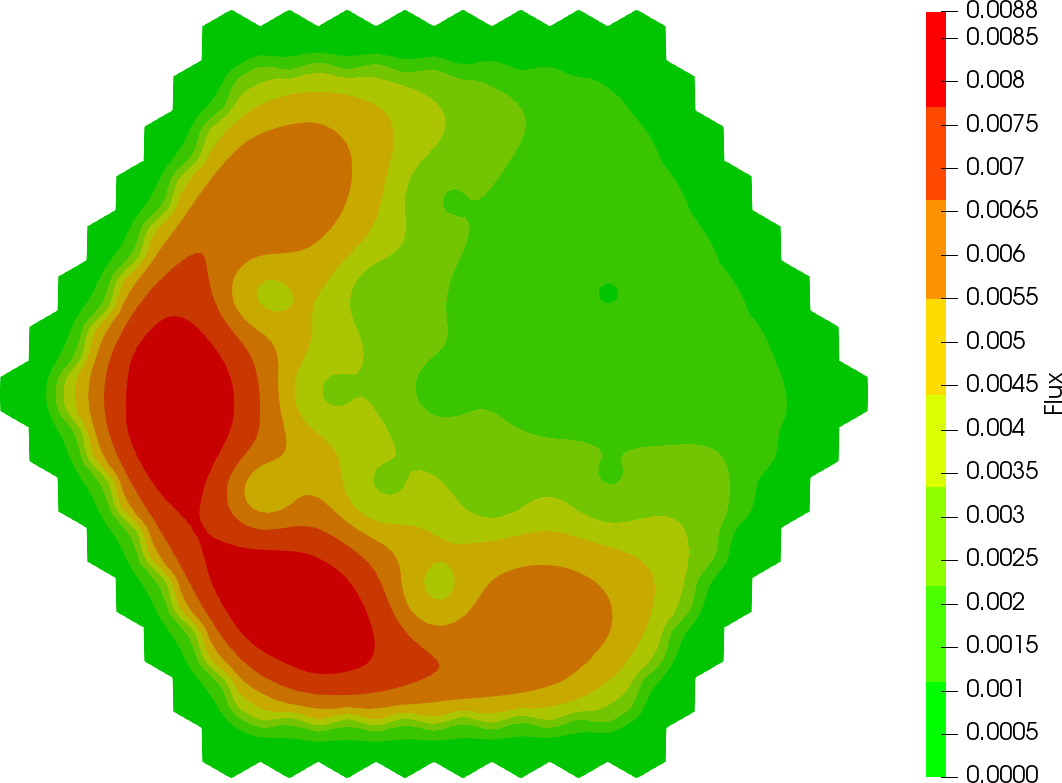
\includegraphics[width=0.49\linewidth]{iaea_cosym/sp3_alpha_u1_1_assym.png}
	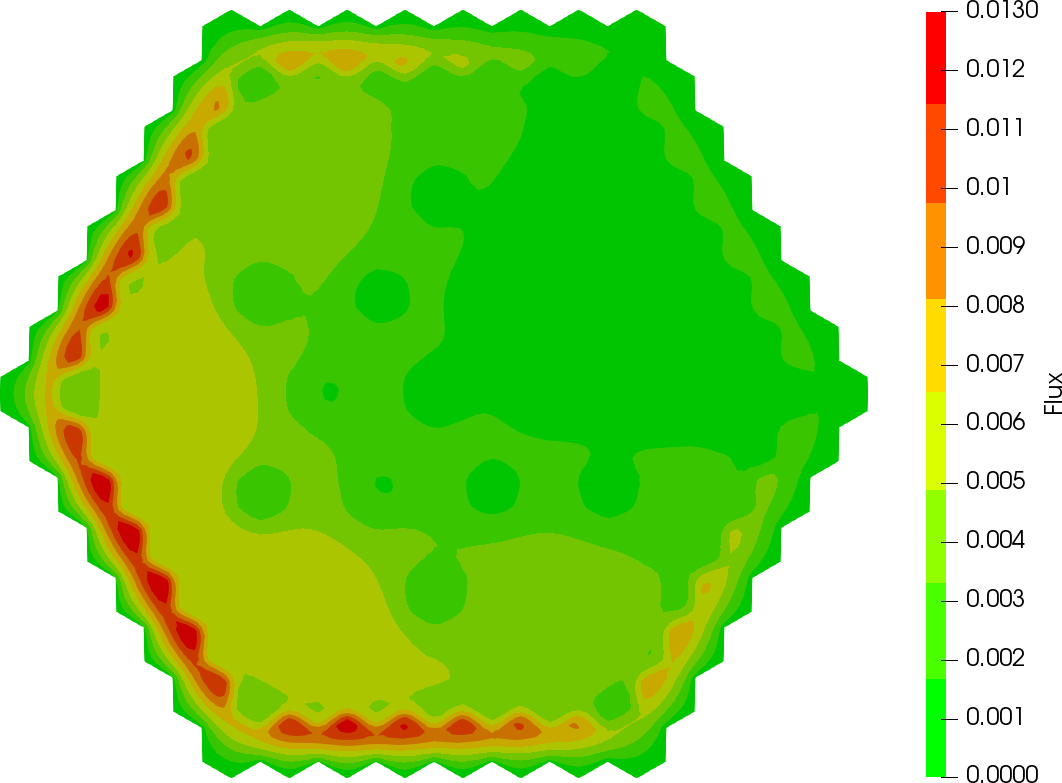
\includegraphics[width=0.49\linewidth]{iaea_cosym/sp3_alpha_u2_1_assym.png}\\
	\caption{Eigenfunctions $\phi_1^{(1)}$, $\phi_2^{(1)}$.}
	\label{fig:iaea_cosym_fun_1}
\end{center}
\end{figure}

\begin{figure}[h]
\begin{center}
	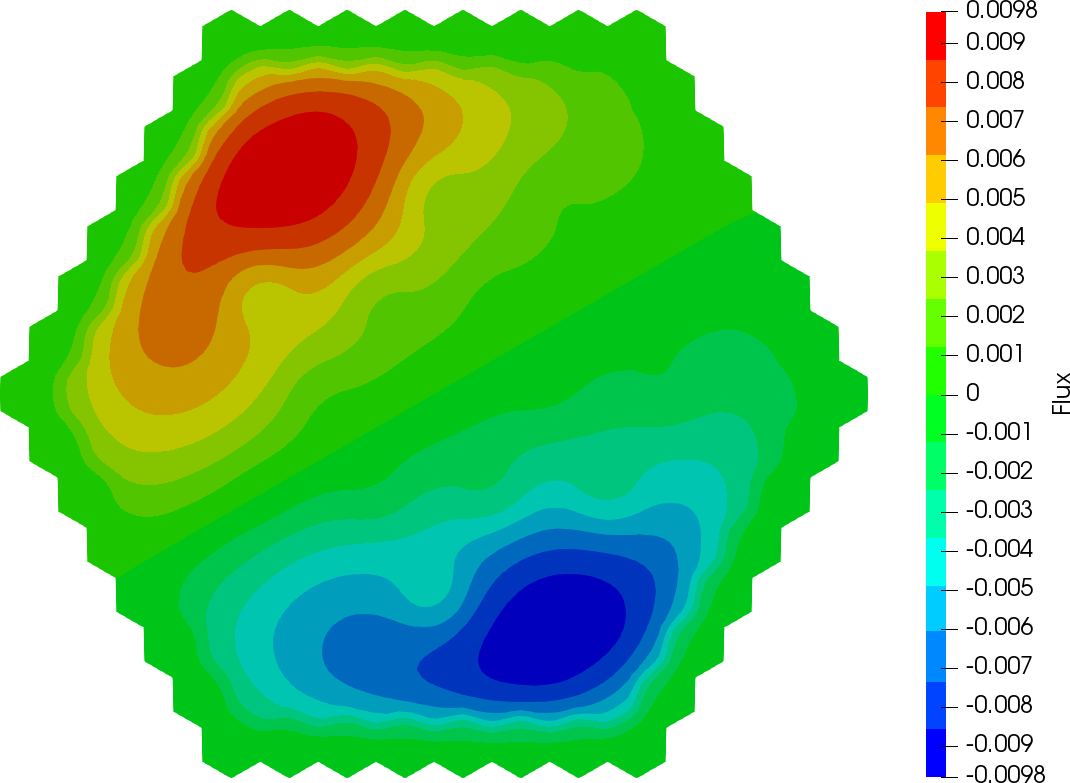
\includegraphics[width=0.49\linewidth]{iaea_cosym/sp3_alpha_u1_2_assym.png}
	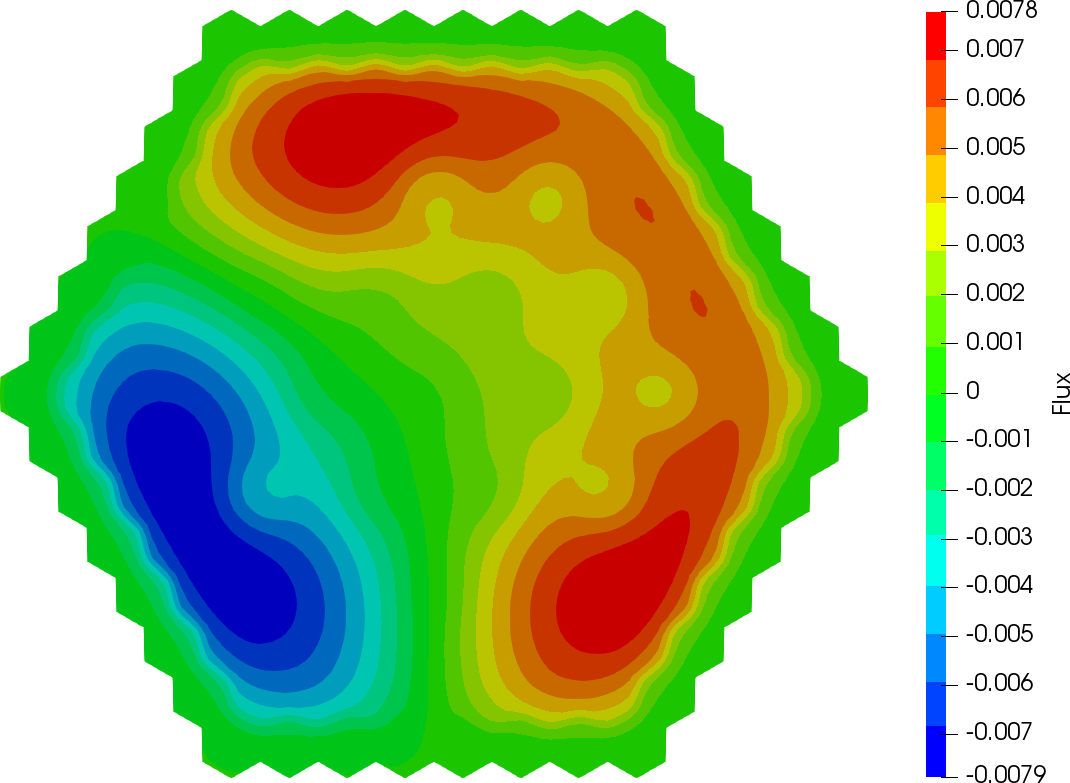
\includegraphics[width=0.49\linewidth]{iaea_cosym/sp3_alpha_u1_3_assym.png}\\
	\caption{Eigenfunctions $\phi_1^{(2)}$, $\phi_1^{(3)}$.}
	\label{fig:iaea_cosym_fun_2}
\end{center}
\end{figure}

\begin{figure}[h]
\begin{center}
	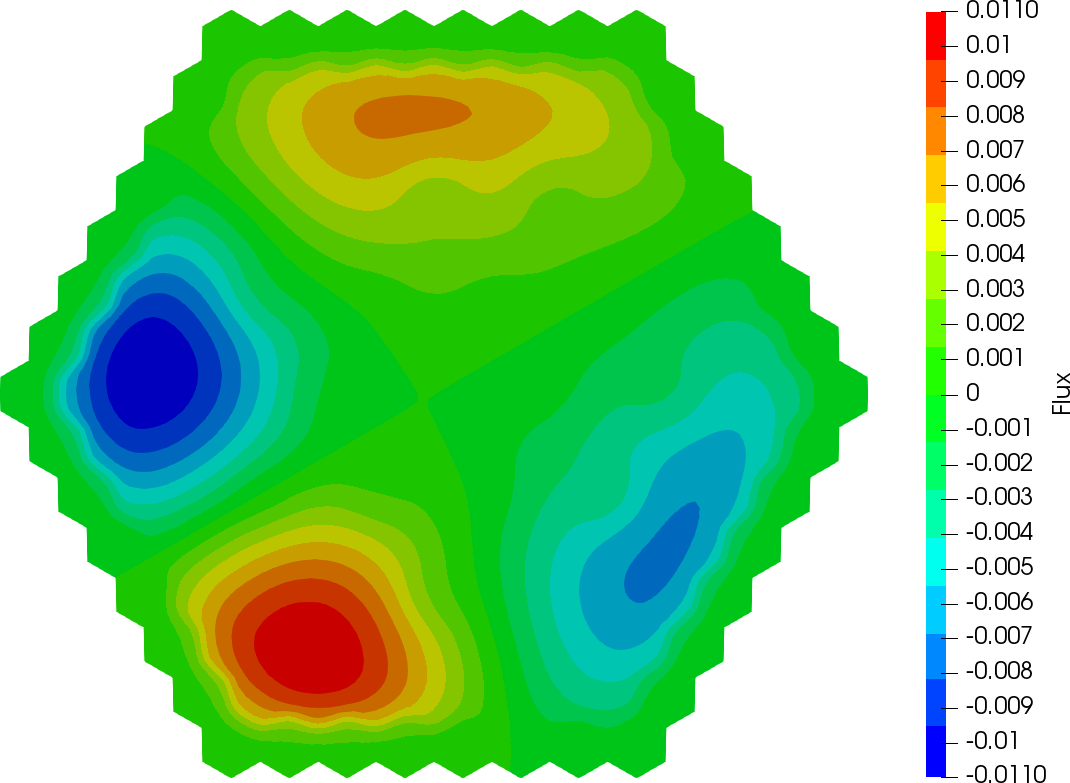
\includegraphics[width=0.49\linewidth]{iaea_cosym/sp3_alpha_u1_4_assym.png}
	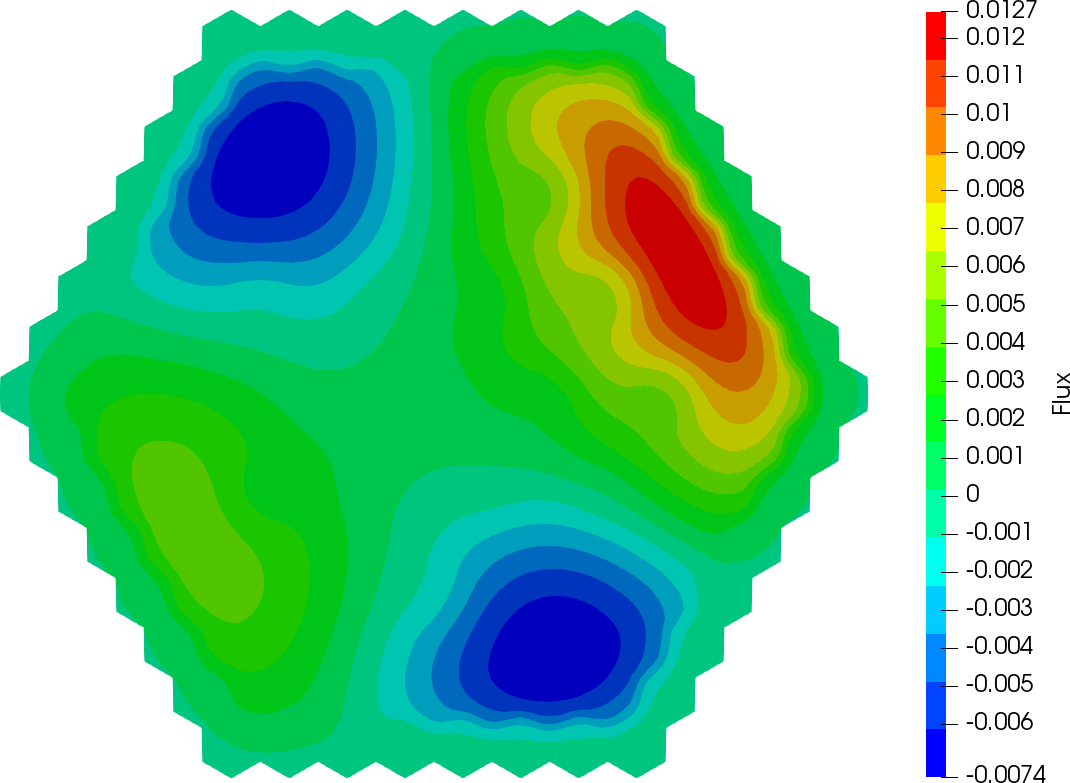
\includegraphics[width=0.49\linewidth]{iaea_cosym/sp3_alpha_u1_5_assym.png}\\
	\caption{Eigenfunctions $\phi_1^{(4)}$, $\phi_1^{(5)}$.}
	\label{fig:iaea_cosym_fun_3}
\end{center}
\end{figure}

\subsection{HWR problem}
This benchmark simulate the active zone of a large heavy-water reactor HWR \citep{chao1995}. 
The geometrical model of the HWR reactor core consists of a set of hexagonal assemblies and is presented in Fig. \ref{fig:hwr}. 
The total size of assembly equals 17.78 cm. Diffusion neutronics constants in the common units are given in Table \ref{tab:hwr}. 

\begin{table}[h]
\caption{Diffusion neutronics constants for HWR.}
\label{tab:hwr}
\begin{center}
\begin{tabular}{ccllll}
\hline
Material & Group & $D$, cm & $\Sigma_r$, cm$^{-1}$ & $\Sigma_{1\to 2}$, cm$^{-1}$ & $\nu\Sigma_f$, cm$^{-1}$\\
\hline
\multirow{ 2}{*}{1} & 1 & 1.38250058 & 1.1105805e-2 & \multirow{ 2}{*}{8.16457e-3} & 2.26216e-3 \\
  & 2 & 0.89752185 & 2.2306487e-2 &            & 2.30623e-2 \\
\hline
\multirow{ 2}{*}{2} & 1 & 1.38255219 & 1.1174585e-2 & \multirow{ 2}{*}{8.22378e-3} & 2.22750e-3 \\
  & 2 & 0.89749043 & 2.2387609e-2 &            & 2.26849e-2 \\
\hline
\multirow{ 2}{*}{3} & 1 & 1.37441741 & 1.0620368e-2 & \multirow{ 2}{*}{8.08816e-3} & 2.14281e-3 \\
  & 2 & 0.88836771 & 1.6946527e-2 &            & 2.04887e-2 \\
\hline
\multirow{ 2}{*}{4} & 1 & 1.31197955 & 1.2687953e-2 & \multirow{ 2}{*}{1.23115e-2} & 0.0 \\
  & 2 & 0.87991376 & 5.2900925e-2 &            & 0.0 \\
\hline
\multirow{ 2}{*}{6} & 1 & 1.38138909 & 1.056312e-2 & \multirow{ 2}{*}{7.76568e-3} & 2.39469e-3 \\
  & 2 & 0.90367052 & 2.190298e-2 &            & 2.66211e-2 \\
\hline
\multirow{ 2}{*}{7} & 1 & 1.30599110 & 1.1731321e-2 & \multirow{ 2}{*}{1.10975e-2} & 0.0 \\
  & 2 & 0.83725587 & 4.3330365e-3 &            & 0.0 \\
\hline
\multirow{ 2}{*}{8} & 1 & 1.29192957 & 1.1915316e-2 & \multirow{ 2}{*}{1.15582e-2} & 0.0 \\
  & 2 & 0.81934103 & 3.0056488e-4 &            & 0.0 \\
\hline
\multirow{ 2}{*}{9} & 1 & 1.06509884 & 2.8346221e-2 & \multirow{ 2}{*}{2.61980e-2} & 0.0 \\
  & 2 & 0.32282849 & 3.3348874e-2 &            & 0.0 \\  
\hline
\end{tabular}
\end{center}
\end{table}

\begin{figure}[hp]
	\begin{center}
    		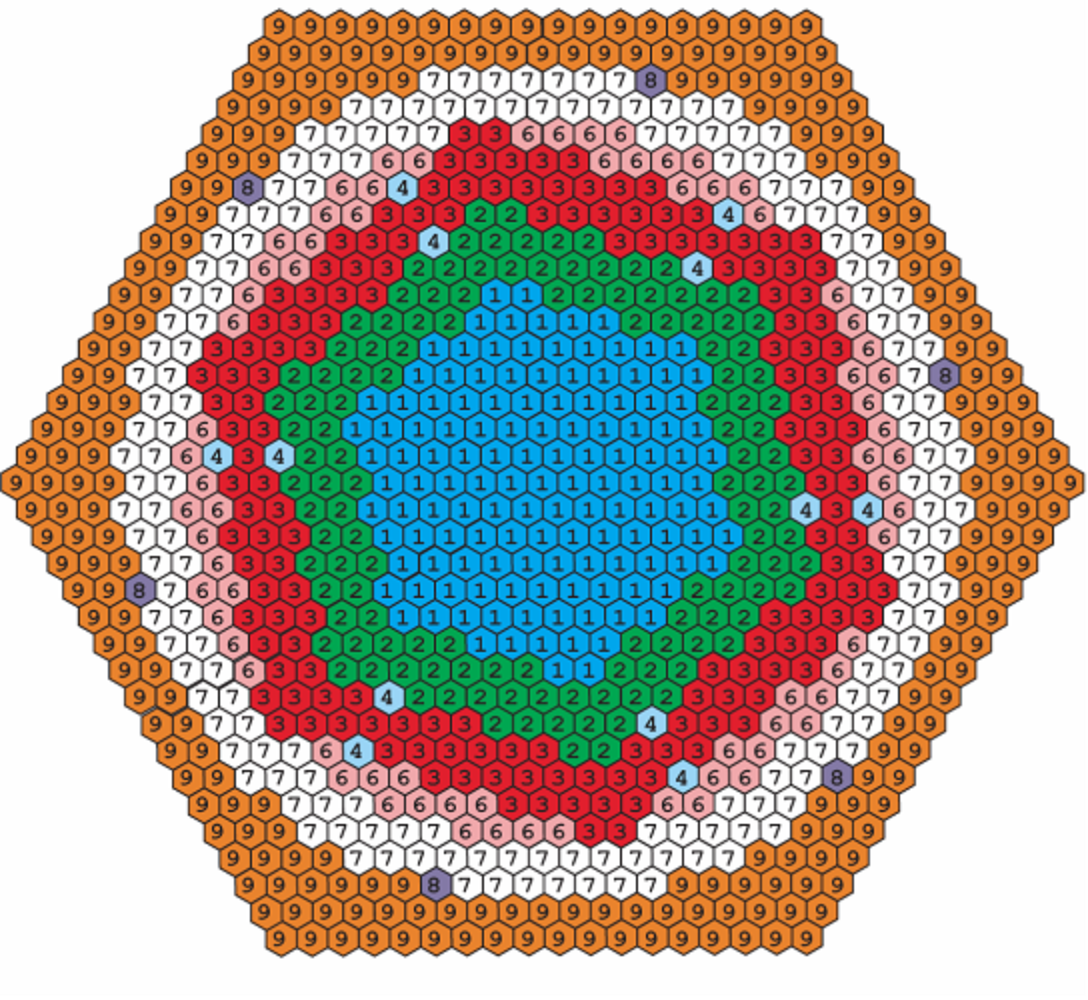
\includegraphics[width=0.9\linewidth] {hwr.png}
		\caption{Geometrcial model of the HWR reactor core.}
		\label{fig:hwr}
	\end{center}
\end{figure} 

\subsubsection{Solution of Lambda Modes spectral problem}
%В качестве эталонного решения по диффузионной модели взято 0.991965\cite{chao1995}, а по транспортной модели взято решение на мелкой сетке при $p=3, n=96$.
%Результаты расчета теста HWR приведены в таблице \ref{tab:hwr_lambda}. 
%В таблице \ref{tab:hwr_lambda_10} приведены результаты первых 10 собственных значений при $p=3, n=96$. 
%Для рассматриваемого теста собственные значения $\alpha_2, \alpha_3$, $\alpha_4, \alpha_5$, $\alpha_9, \alpha_{10}$ являются комплексными с малой мнимой частью, собственные значения $\alpha_1, \alpha_6$, $\alpha_7, \alpha_8$ --- действительными.

\begin{table}[h]
\caption{The effective multiplication factor.}
\label{tab:hwr_lambda}
\begin{center}
\begin{tabular}{c c r r r r r r}
\hline
$n$ & $p$ & $k_{dif}$ & $\Delta_{dif}$ & $\delta_{dif}$ &$k_{sp_3}$& $\Delta_{sp_3}$ & $\delta_{dif}$ \\
\hline
	& 1	& 0.991985&  2.0& 1.16&0.992178&   5.0& 0.80\\
6	& 2	& 0.991989&  2.4& 0.31&0.992166&   3.8& 0.24\\
	& 3	& 0.991964&  0.1& 0.08&0.992132&   0.4& 0.07\\
\hline
	& 1	& 0.991983&  1.8& 0.05&0.992165&   3.7& 0.08\\
24& 2	& 0.991965&  0.0& 0.01&0.992133&   0.5& 0.01\\
	& 3	& 0.991963&  0.2& 0.01&0.992128&   0.0& 0.00\\ 
\hline
	& 1	& 0.991969&  0.4& 0.08&0.992140&   1.2& 0.01\\
96& 2	& 0.991963&  0.2& 0.02&0.992129&   0.1& 0.00\\
	& 3	& 0.991963&  0.2& 0.01&0.992128&    --& --\\ 
\hline
Ref.&   & 0.991965&    & & 0.992128 & & \\ 
\hline
\end{tabular}
\end{center}
\end{table}

\begin{table}[h]
\caption{The eigenvalues $k_i=1/\lambda_i^{(k)}$ for $p=3, n=96$.}
\label{tab:hwr_lambda_10}
\begin{center}
\begin{tabular}{c l l }
\hline
$i$ & diffusion & SP$_3$  \\
\hline
1 & 0.99196 + 0.0$i$   & 0.99213 + 0.0$i$\\
2 & 0.98359 + 1.1645e-05$i$   & 0.98379 + 1.2072e-05$i$\\
3 & 0.98359 $-$ 1.1645e-05$i$ & 0.98379 $-$ 1.2072e-05$i$\\
4 & 0.96424 + 2.1564e-05$i$   & 0.96452 + 2.2337e-05$i$\\
5 & 0.96424 $-$ 2.1564e-05$i$ & 0.96452 $-$ 2.2337e-05$i$\\
6 & 0.94329 + 0.0$i$   & 0.94373 + 0.0$i$\\
7 & 0.92387 + 0.0$i$   & 0.92426 + 0.0$i$\\
8 & 0.91866 + 0.0$i$   & 0.91880 + 0.0$i$\\
9 & 0.89568 + 3.5570e-05$i$   & 0.89632 + 3.6750e-05$i$\\
10 & 0.89568 $-$ 3.5570e-05$i$& 0.89632 + 3.6750e-05$i$\\
\hline
\end{tabular}
\end{center}
\end{table}

\subsubsection{Solution of Alpha Modes spectral problem}
As a reference solution, the solutions obtained using the diffusion or transport model on a fine grid $ p = 3, n = 96 $ are taken.

\textbf{Without delayed neutrons.}

%В таблице \ref{tab:hwr_alpha} показаны результаты расчета $\alpha$-спектральной задачи без учета запаздывающих нейтронов при использовании различных сеток и конечных элементов. Эти данные демонстрируют сходимость приближенно вычисляемых собственных значений при сгущении сетки $n$ и при увеличении степени аппроксимирующих полиномов $p$. 
%В таблице \ref{tab:hwr_alpha_10} приведены результаты первых десяти собственных значений $\alpha$-спектральной задачи при мелкой сетке $p=3, n=96$. 
%Сами собственные значения   $\mathrm{Re}\lambda_1^{(\alpha)} \leq \mathrm{Re}\lambda_2^{(\alpha)} \leq ...$ хорошо отделены друг от друга.
%В данном случае собственные значения $\alpha_2, \alpha_3$, $\alpha_4, \alpha_5$, $\alpha_8, \alpha_{9}$ являются комплексными с малой мнимой частью, собственные значения $\alpha_1, \alpha_6$, $\alpha_7, \alpha_{10}$ --- действительными.
%На рисунках \ref{fig:hwr_fun_1}, \ref{fig:hwr_fun_2}, \ref{fig:hwr_fun_3} показаны собственные функции для SP$_3$ модели.

\begin{table}[h]
\caption{The period eigenvalues.}
\label{tab:hwr_alpha}
\begin{center}
\begin{tabular}{rrrrrr}
\hline
$n$ & $p$ & $\alpha_{dif}$ & $\Delta_{dif}$ &$\alpha_{sp_3}$& $\Delta_{sp_3}$ \\
\hline
	& 1	&42.281 & 0.018 & 41.246 & 0.134\\
6	& 2	&42.135 & 0.128 & 41.190 & 0.190\\
	& 3	&42.259 & 0.004 & 41.362 & 0.018\\ 
\hline
	& 1	&42.196 & 0.067 & 41.228 & 0.152\\
24& 2	&42.253 & 0.010 & 41.354 & 0.026\\
	& 3	&42.263 & 0.000 & 41.379 & 0.001\\ 
\hline
	& 1	&42.241 & 0.022 & 41.330 & 0.050\\
96& 2	&42.262 & 0.001 & 41.377 & 0.003\\
	& 3	&42.263 &    -- & 41.380 & -- \\ 
\hline
Ref.& & 42.263 & & 41.380 \\ 
\hline
\end{tabular}
\end{center}
\end{table}

\begin{table}[h]
\caption{The eigenvalues $\alpha_i=\lambda_i^{(\alpha)}$ for $p=3, n=96$.}
\label{tab:hwr_alpha_10}
\begin{center}
\begin{tabular}{c l l}
\hline
$i$ & Diffusion & SP$_3$ \\
\hline
1 &\phantom{0}42.263 + 0.0$i$       &41.380 + 0.0$i$ \\
2 &\phantom{0}84.867 $-$ 0.06130$i$ &83.821 $-$ 0.06358$i$ \\
3 &\phantom{0}84.867 + 0.06130$i$   &83.821 + 0.06358$i$ \\
4 &182.914 $-$ 0.11367$i$           &181.471 $-$ 0.11805$i$ \\
5 &182.914 + 0.11367$i$             &181.471 + 0.11805$i$ \\
6 &293.017 + 0.0$i$                 &290.940 + 0.0$i$ \\
7 &371.528 + 0.0$i$                 &369.374 + 0.0$i$ \\
8 &515.465 $-$ 0.16397$i$           &512.337 $-$ 0.17197$i$ \\
9 &515.465 + 0.16397$i$             &512.337 + 0.17197$i$ \\
10&518.670 + 0.0$i$                 &517.975 + 0.0$i$ \\
\hline
\end{tabular}
\end{center}
\end{table}

\begin{figure}[h]
\begin{center}
	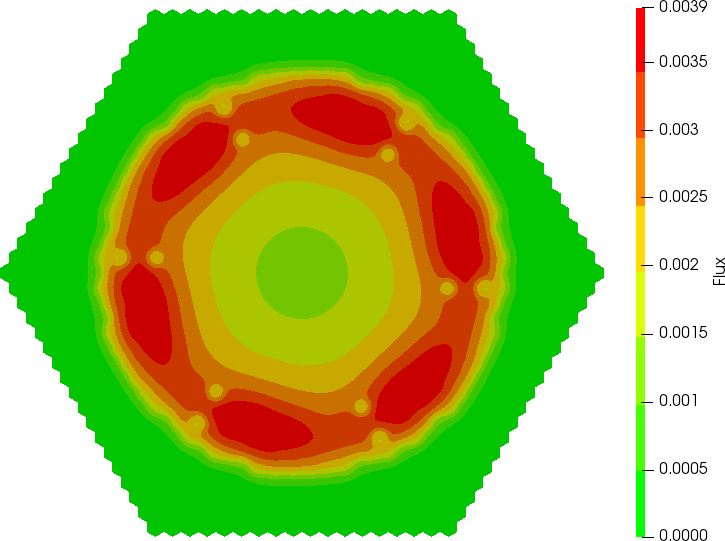
\includegraphics[width=0.49\linewidth]{hwr/alpha_sp3_rx1_1.png}
	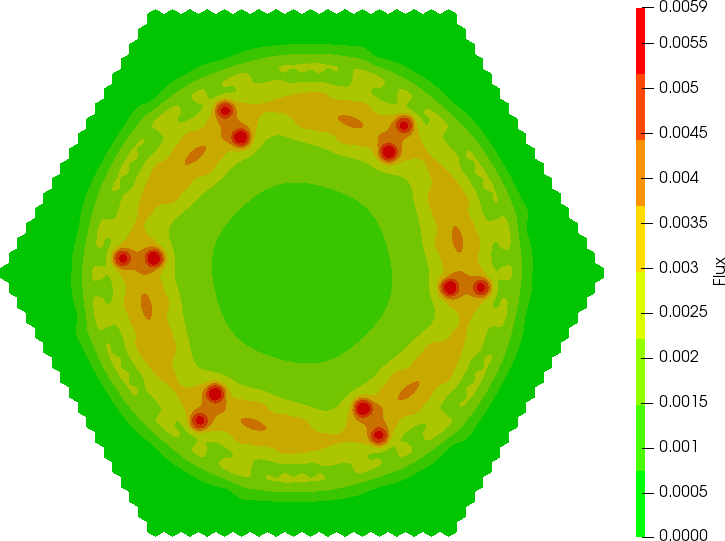
\includegraphics[width=0.49\linewidth]{hwr/alpha_sp3_rx2_1.png}\\
	\caption{The eigenfunctions $\phi^{(1)}_1$ (left) and $\phi^{(1)}_2$ (right).}
	\label{fig:hwr_fun_1}
\end{center}
\end{figure}

\begin{figure}[h]
\begin{center}
	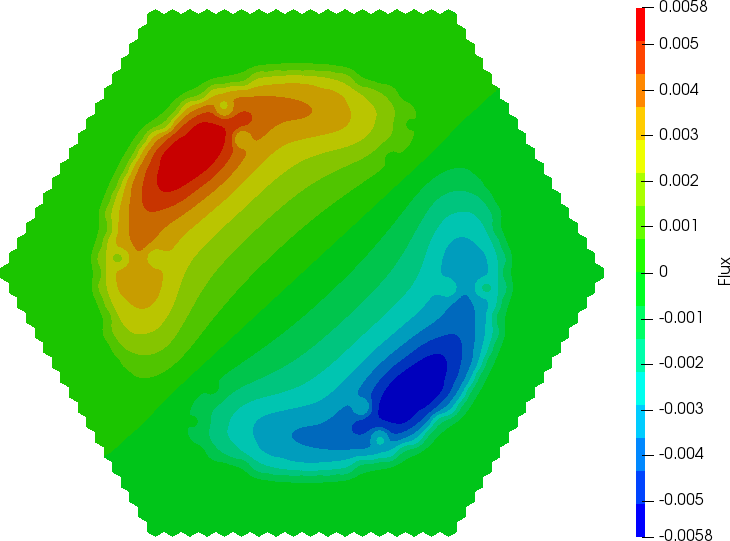
\includegraphics[width=0.49\linewidth]{hwr/alpha_sp3_rx1_2.png}
	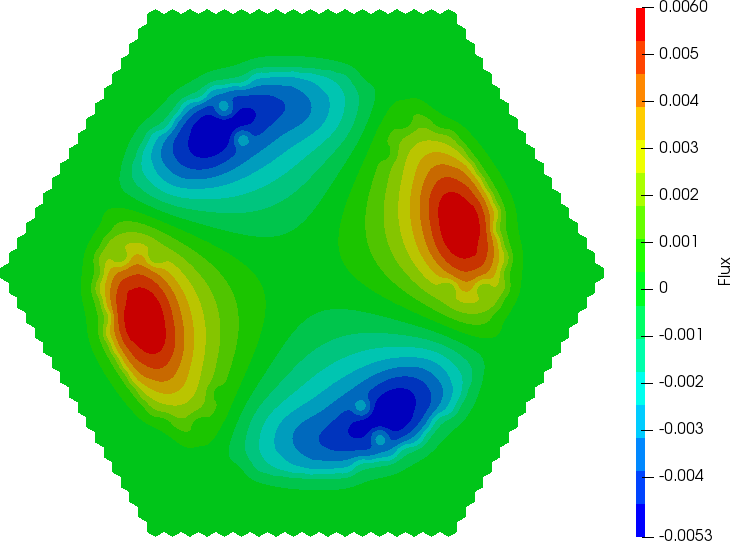
\includegraphics[width=0.49\linewidth]{hwr/alpha_sp3_rx1_4.png}\\
	\caption{Real part of eigenfunctions $\phi^{(2)}_1, \ \phi^{(3)}_1$ (left) and $\phi^{(4)}_1, \ \phi^{(5)}_1$ (right).}
	\label{fig:hwr_fun_2}
\end{center}
\end{figure}

\begin{figure}[h]
\begin{center}
	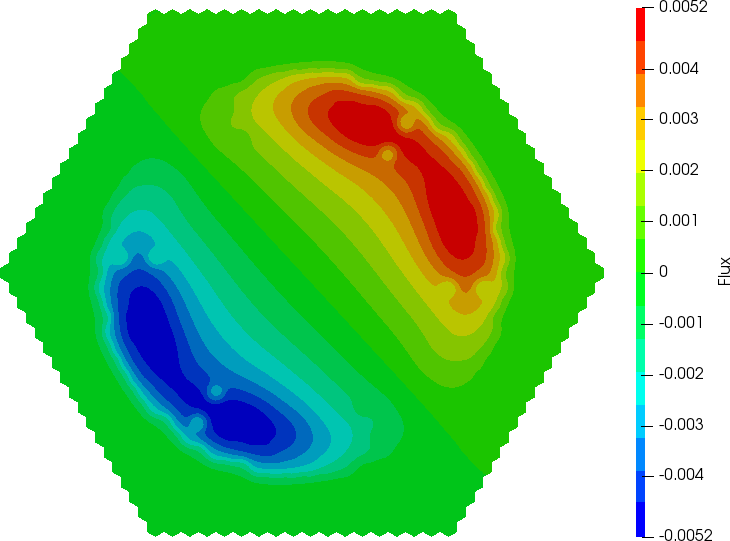
\includegraphics[width=0.49\linewidth]{hwr/alpha_sp3_cx1_2.png}
	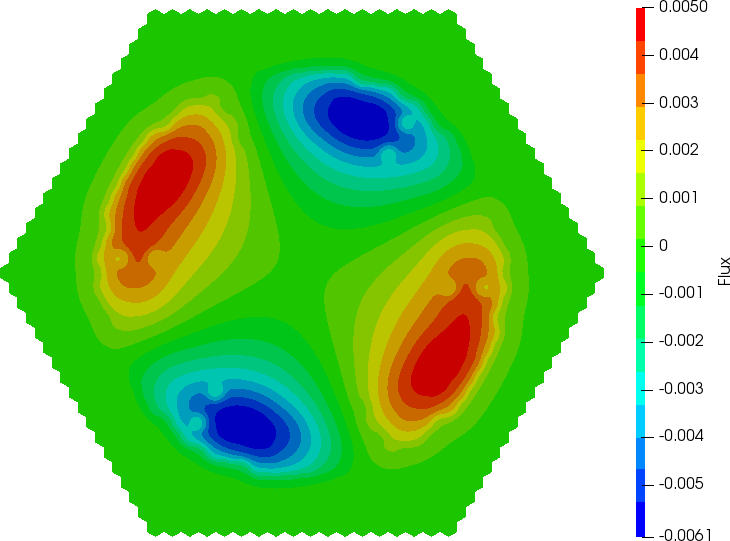
\includegraphics[width=0.49\linewidth]{hwr/alpha_sp3_cx1_4.png}\\
	\caption{Imaginary part of eigenfunctions $\phi^{(2)}_1, \ - \phi^{(3)}_1$ (left) and $\phi^{(4)}_1, \ - \phi^{(5)}_1$ (right).}
	\label{fig:hwr_fun_3}
\end{center}
\end{figure}

\textbf{With delayed neutrons.}

\begin{table}[h]
\caption{The period eigenvalues.}
\label{tab:hwr_alpha_del}
\begin{center}
\begin{tabular}{rrrrrr}
\hline
$n$ & $p$ & $\alpha_{dif}$ & $\Delta_{dif}$ &$\alpha_{sp_3}$& $\Delta_{sp_3}$ \\
\hline
	& 1	&0.04431 & 0.00006 & 0.04383 & 0.00012\\
6	& 2	&0.04430 & 0.00007 & 0.04386 & 0.00009\\
	& 3	&0.04437 & 0.00000 & 0.04394 & 0.00001\\ 
\hline
	& 1	&0.04432 & 0.00005 & 0.04386 & 0.00009\\
24& 2	&0.04436 & 0.00001 & 0.04394 & 0.00001\\
	& 3	&0.04437 & 0.00000 & 0.04395 & 0.00000\\ 
\hline
	& 1	&0.04435 & 0.00002 & 0.04392 & 0.00003\\
96& 2	&0.04437 & 0.00000 & 0.04395 & 0.00000\\
	& 3	&0.04437 & --      & 0.04395 & -- \\ 
\hline
Ref.& & 0.04437 & & 0.04395 \\ 
\hline
\end{tabular}
\end{center}
\end{table}

\begin{table}[h]
\caption{The eigenvalues $\alpha_i=\lambda_i^{(\alpha)}$ for $p=3, n=96$.}
\label{tab:hwr_alpha_del_10}
\begin{center}
\begin{tabular}{c l l}
\hline
$i$ & Diffusion & SP$_3$ \\
\hline
1 &0.04437 + 0.0$i$     		&0.04395 + 0.0$i$ \\
2 &0.05755 $-$ 1.15549e-05$i$ 	&0.05735 $-$ 1.22333e-05$i$ \\
3 &0.05755 + 1.15549e-05$i$   	&0.05735 + 1.22333e-05$i$ \\
4 &0.06807 $-$ 6.35264e-06$i$   &0.06798 $-$ 6.66947e-06$i$ \\
5 &0.06807 + 6.35264e-06$i$     &0.06798 + 6.66947e-06$i$ \\
6 &0.07219 + 0.0$i$             &0.07213 + 0.0$i$ \\
7 &0.07415 + 0.0$i$             &0.07412 + 0.0$i$ \\
8 &0.07453 + 0.0$i$          	&0.07452 + 0.0$i$ \\
9 &0.07577 $-$ 1.52484e-06$i$   &0.07574 $-$ 1.60360e-06$i$ \\
10&0.07577 + 1.52484e-06$i$     &0.07574 + 1.60360e-06$i$ \\
\hline
\end{tabular}
\end{center}
\end{table}

\pagebreak
\newpage
\section*{Acknowledgements}

This work was supported by the Russian Foundation for Basic Research (\#~18-31-00315) 
and by the grant of the Russian Federation Government (\#~14.Y26.31.0013).

\section*{Reference}
\bibliography{sp3}

\end{document}
